\documentclass[times, utf8, zavrsni, numeric]{fer}
\usepackage{booktabs}
\usepackage{url}
\usepackage{siunitx}
\usepackage{listings}
\usepackage{graphicx}
\usepackage{caption}
\usepackage{subcaption}
\usepackage[export]{adjustbox}
\usepackage{float}



\begin{document}

% Ukljuci literaturu
\nocite{*}

\thesisnumber{6647}

\title{Model dijela grada Zagreba temeljen na realnim podacima}

\author{Luka Mesarić}

\maketitle

\izvornik

\zahvala{}

\tableofcontents

\counterwithout*{footnote}{chapter}

\renewcommand{\lstlistingname}{Algoritam}
\lstset{language=Python, basicstyle=\footnotesize, numbers=left}



\chapter{Uvod}
	
	Izrada trodimenzionalnih modela gradova svoju primjenu nalaze u mnogim područjima ljudske djelatnosti.
	U eri svekolike digitalizacije i nagle urbanizacije mapiranje terena omogućuje učinkovito urbanističko planiranje s ciljem boljeg razumijevanja i upravljanja urbanim ekosustavima u smjeru razvoja pametnih gradova.
	
	Inteligentna rješenja transportnih i evakuacijskih puteva u slučaju prirodnih katastrofa, organizacija cestovnog i zračnog prometa, raspoređivanje telekomunikacijskih odašiljača i slično samo su neka od područja primjene modela gradova.
	Također se koriste u vizualizaciji postupka kontrole prometa postavljanjem nadzornih kamerama, planiranju osvijetljenosti cesta kao i cijelih stambenih područja~\cite{biljeckimodels}.
	
	Ne manje važna je i mogućnost raspoređivanja zelenih i vodenih površina, prostorna analiza i simulacija insolacije radi optimalnog pozicioniranja solarnih kolektora, praćenje izmjene perioda zasjenjenosti i osunčanosti zgrada s ciljem upravljanja potrebama za energentima.
	
	U seizmički aktivnim područjima važna je projekcija oštećenja zgrada od potresa kao i učinak rušenja na okolne objekte, a u regijama s jakim vjetrovima trodimenzionalni modeli od velike su pomoći u arhitekturi visokih zgrada.
	
	U velikim i gusto naseljenim područjima od osobite je važnosti mogućnost praćenja urbanih zagađivača, primjerice isijavanje topline s pločnika i kolnika u međuprostorima zgrada, analiza količine urbane buke i vidljivosti neba između nebodera.
	
	Vojni i sigurnosni segmenti također su zastupljeni u području primjene trodimenzionalnih modela pri čemu modele koriste za obuku kadra i simulaciju kretanja.
	
	U multimediji trodimenzionalne simulacije gradova nude brojne mogućnosti u dizajnu video igara, filmskoj industriji i oglašavanju.  
	
	U turističkom sektoru i zaštiti kulturne baštine modeli gradova služe boljoj vizualnoj prepoznatljivosti lokacije i kreiranju virtualnih razgleda.
	
	\eject
	
	U ovom radu razmatra se postupak automatskog generiranja trodimenzionalnog modela proizvoljnog dijela grada Zagreba  temeljenog na realnim i javno dostupnim podatcima.
	
	Model se izrađuje u omjeru $1:1$ te se realistično prikazuje teren, zgrade i stabla.
	Područje za koje se planira generirati trodimenzionalni model zadaje se geografskim koordinatama donjeg lijevog i gornjeg desnog ugla. 
	Posljedično, područje mora biti pravokutnog oblika.
	
	Za izradu modela koristi se dodatak za alat \textit{Blender} napisan u programskom jeziku \textit{Python}.



\chapter{Korištene tehnologije i alati}

	\section{Blender}

		Konačno programsko rješenje razvijeno u ovom radu jest dodatak \engl{add-on} za \textit{Blender},\footnote{\url{https://www.blender.org/}} profesionalni programski alat otvorenog kôda namijenjen za 3D računalnu grafiku.
		Između ostalog, alat \textit{Blender} koristi se za 3D modeliranje, animiranje objekata i stvaranje animiranih filmova, izradu vizualnih efekata, simuliranje fluida i čestičnih sustava te izrađivanje prikaza 3D scena \engl{rendering}.
		
		Za razvoj programskog rješenja korišten je \textit{Blender} verzije $2.82$ te je ista ili novija verzija potrebna za instalaciju i pokretanje dodatka.
	
	
	
	\section{Python}

		Programsko rješenje razvijeno je koristeći programski jezik \textit{Python}.\footnote{\url{https://www.python.org/}}
		\textit{Blender} verzije $2.82$ uključuje interpreter za \textit{Python} verzije $3.7.4$, te je stoga programski kôd pisan u istoj verziji.
		
		Programsko obavljanje operacija u \textit{Blenderu} omogućeno je kroz \textit{Python} API i posebne module, primarno \texttt{bpy}, \texttt{bmesh} i \texttt{mathutils}.\footnote{\url{https://docs.blender.org/api/current/}}
	
	
	
	\section{Dodatne biblioteke} \label{custom_libraries}
	
		Osim biblioteka uključenih u standardnu instalaciju \textit{Pythona}, prilikom razvoja programskog rješenja upotrijebljeno je nekoliko javno dostupnih biblioteka trećih strana.
		
		Biblioteka \textit{Requests: HTTP for Humans™} služi vrlo jednostavnom slanju HTTP zahtjeva.\footnote{\url{https://requests.readthedocs.io/}}
		Za razvoj se koristi stabilna verzija $2.23.0$.
		
		Biblioteka \textit{Pillow} proširenje je biblioteke PIL (\textit{Python Imaging Library}) te služi za obradu slika.\footnote{\url{https://pillow.readthedocs.io/}}
		Prilikom razvoja korištena je verzija $7.1.2$.
	
		Biblioteka \textit{pyproj} sučelje je za programski jezik \textit{Python} prema biblioteci PROJ za kartografske projekcije i transformacije koordinata.\footnote{\url{https://pyproj4.github.io/pyproj/}}
		Korištena je verzija $2.6.1$.
	
	
	
	\section{Unreal Engine}

		\textit{Unreal Engine} grafički je programski pogon otvorenog kôda pisan u programskom jeziku \textit{C++}.\footnote{\url{https://www.unrealengine.com/}}
		Razvija ga tvrtka \textit{Epic Games}.
		Za prikaz modela kojeg generira \textit{Blender} dodatak koristi se \textit{Unreal Engine} verzije $4.22.3$.
		
		Iako je programsko rješenje za izradu modela moglo biti izvedeno i kao dodatak za \textit{Unreal Engine}, ipak je odabran \textit{Blender} radi lakšeg razvoja.
		Naime, za razliku od programskog jezika \textit{C++}, jezik \textit{Python} pogodniji je za mnoge operacije koje su ključne pri izgradnji modela, poput mrežne komunikacije.
		S druge strane, program napisan u jeziku \textit{C++} nedvojbeno bi se brže izvodio.
		Međutim, to nije presudno jer se model grada izrađuje samo jednom nakon čega se može neograničeno koristiti s obzirom na to da se zapravo radi samo o jednostavnom skupu objekata.



\chapter{Instalacija i korištenje razvijenog dodatka}

	Razvijeno programsko rješenje prije korištenja potrebno je instalirati kao dodatak u alatu \textit{Blender}.
	Sav izvorni kôd sprema se u ZIP arhivu iz koje \textit{Blender} stvara i registrira novi dodatak.
	
	U alatu \textit{Blender} slijedom klikova na gumbe \texttt{Edit > Preferences > Add-ons > Install} otvara se preglednik datoteka na računalu.
	Nakon lociranja ZIP arhive odabire se "\textit{Install Add-on}" i označuje kućica \engl{checkbox} pored imena dodatka u njegovim postavkama (slika \ref{fig:install_dependencies_button}).\footnote{\url{https://docs.blender.org/manual/en/latest/advanced/scripting/addon_tutorial.html#install-the-add-on}}
	Time je dodatak instaliran i registriran te postaje aktivan u grafičkom sučelju.
	
	\textit{Blender} koristi vlastitu instalaciju \textit{Python} interpretera i pripadnih biblioteka te je u skriptama i dodatcima moguće koristiti jedino biblioteke koje se nalaze unutar te instalacije.
	Radi olakšanja korištenja dodatka, biblioteke opisane u poglavlju \ref{custom_libraries} o kojima dodatak ovisi automatski se preuzimaju i instaliraju unutar \textit{Blenderove} instalacije \mbox{\textit{Pythona}} pritiskom na gumb "\textit{Install dependencies}" u postavkama dodataka (slika \ref{fig:install_dependencies_button}).
	Za razvoj te funkcionalnosti modificirano je postojeće programsko rješenje~\cite{github:gutzkow}.
	
	\begin{figure}
		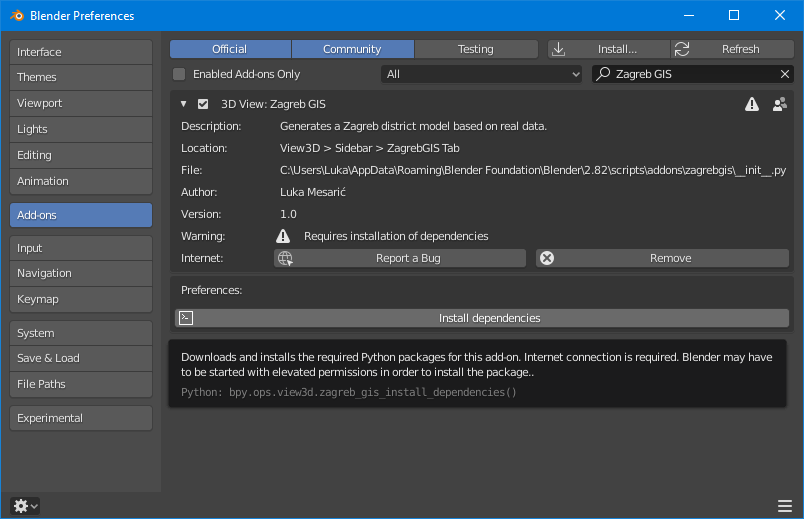
\includegraphics[width=\linewidth]{figures/install_dependencies_button.png}
		\centering
		\caption{Postavke instaliranog dodatka u alatu \textit{Blender}}
		\label{fig:install_dependencies_button}
	\end{figure}
	
	Jednom kada je instalacija dovršena dodatak je moguće koristiti pritiskom na tipku "\texttt{N}" na tipkovnici čime se otvara bočna izborna traka \engl{sidebar} u kojoj se nalazi nova kartica \engl{tab} pod imenom ZagrebGIS.
	Izgled grafičkog sučelja prikazan je na slikama \ref{fig:addon_gui} i \ref{fig:install_dependencies_warning}.
	
	\begin{figure}[ht]
		\centering
		\begin{subfigure}[t]{.317\textwidth}
			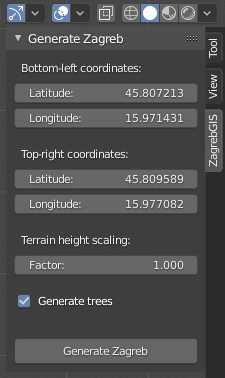
\includegraphics[width=\linewidth,left]{figures/addon_gui.png}
			\captionsetup{margin=.4cm}
			\caption{Instalirane biblioteke}
			\label{fig:addon_gui}
		\end{subfigure}
		\hfill
		\begin{subfigure}[t]{.67\textwidth}
			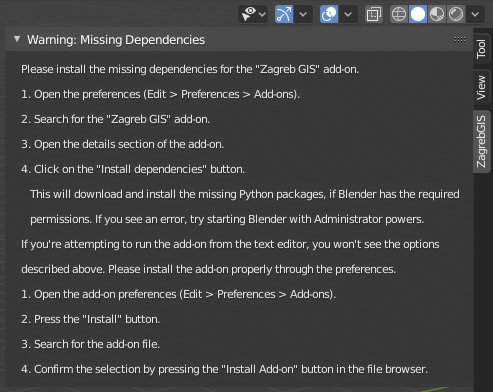
\includegraphics[width=\linewidth,right]{figures/install_dependencies_warning.png}
			\captionsetup{margin=.4cm}
			\caption{Biblioteke nedostaju}
			\label{fig:install_dependencies_warning}
		\end{subfigure}
		\caption{Grafičko sučelje dodatka ZagrebGIS}
		\label{fig:addon_gui_examples}
	\end{figure}



\chapter{Teren}

	\section{Visinska mapa}
	
		Visinska mapa \engl{heightmap} posebna je vrsta slike koja se u 3D grafici koristi za pohranjivanje podataka o visini točaka u trodimenzionalnom prostoru~\cite{jankovic2010}.
		
		Najjednostavnije visinske mape slike su koje sadrže samo jedan kanal boje koji predstavlja udaljenost pojedine točke od referentne razine, odnosno visinu točke.
		Pri tome se crna boja koristi za oznaku najniže, dok bijela boja predstavlja najvišu poziciju.
		U jednoj mapi nije nužno koristiti cijeli raspon boja.
		Primjer visinske mape koja pokriva područje Zagreba veličine približno \SI{20}{\kilo\meter}~$\times$~\SI{20}{\kilo\meter} nalazi se na slici \ref{fig:heightmap_full_zagreb}.
		
		\begin{figure}
			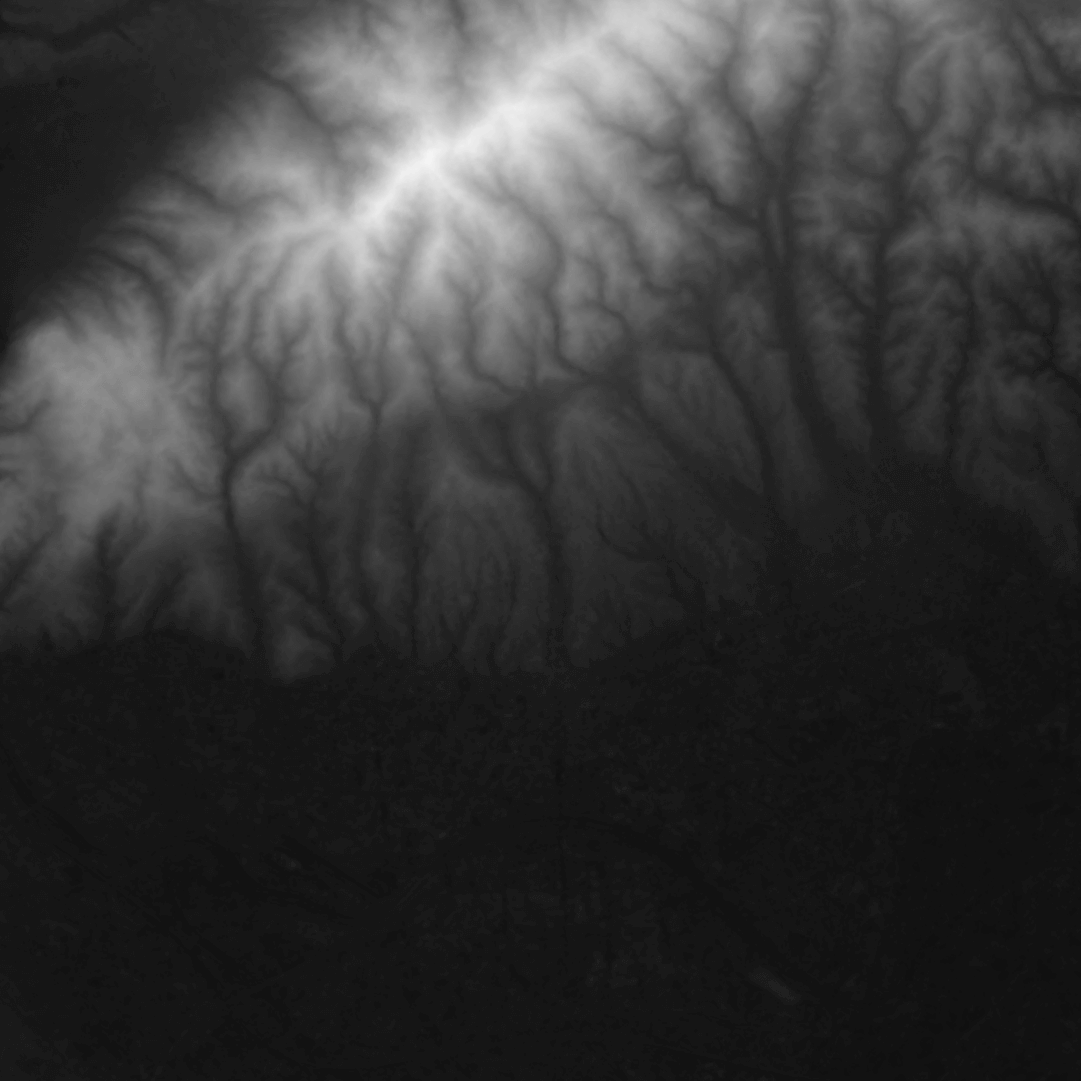
\includegraphics[width=10cm]{figures/heightmap_zagreb_8bit.png}
			\centering
			\caption{Visinska mapa Zagreba i dijela Medvednice preuzeta s \textit{terrain.party}}
			\label{fig:heightmap_full_zagreb}
		\end{figure}
		
		Točnost podataka ovisi o broju bitova po kanalu slike.
		Ako se koristi samo jedan $8$-bitni kanal, moguće je prikazati svega $256$ različitih visina zbog čega se na terenu mogu vidjeti oštre granice poput stepenica.
		S druge strane, u slučaju jednog $16$-bitnog kanala, broj razina povećava se na čak \SI{65536}{}.
		Na primjer, za raspon visine od \SI{1024}{\meter}, koji ugrubo odgovara području Zagreba i Medvednice, sa $16$ bitova po kanalu moguće je prikazati $64$ visinske razine po jednom metru, odnosno jednu razinu svakih \SI{1.56}{\centi\meter}.
	
	
	
	\section{Mapiranje Zemljine površine}
	
		SRTM (\textit{Shuttle Radar Topography Mission}) internacionalni je istraživački projekt koji je rezultirao digitalnim modelom elevacije Zemljine površine od \ang{60} sjeverne do \ang{56} južne geografske širine izrađenim na temelju radarskih snimaka iz \textit{Space Shuttlea Endeavour}.
		Rezolucija mapa jest \SI{30}{\meter} nad područjem Sjedinjenih Američkih Država te \SI{90}{\meter} nad ostalim dijelovima~\cite{wiki:srtm}.
		
		Japanski senzor ASTER (\textit{Advanced Spaceborne Thermal Emission and Reflection Radiometer}) korišten je u najnovijem NASA-inom globalnom istraživanju i mapiranju visinskih podataka o površini Zemlje.\footnote{\url{https://asterweb.jpl.nasa.gov/gdem.asp}}
		Satelitskim snimanjem pokriveno je područje od \ang{83} sjeverne do \ang{83} južne geografske širine, odnosno \SI{99}{\percent} površine kopna, s rezolucijom od \SI{30}{\meter} nad cijelim područjem~\cite{wiki:aster}.
		Glavni je nedostatak to što je instrument sklon pogreškama u slučaju visoke koncentracije oblaka ili naglih promjena u visini čime nastaju rupe u podatcima koje se često moraju ručno popravljati.
	
	
	
	\section{Visinski podatci za područje Zagreba}
	
		Za potrebe ovog rada visinske mape preuzimaju se s besplatne web-aplikacije \textit{terrain.party}\footnote{\url{https://terrain.party/}} koja je originalno razvijena za potrebe simulacijske igre \textit{Cities: Skylines}.\footnote{\url{https://www.citiesskylines.com/}}
		
		Visinske mape koje aplikacija generira crno-bijele su slike rezolucije $1081$~$\times$~$1081$ piksela u formatu PNG (\textit{Portable Network Graphics}) s jednim $16$-bitnim kanalom.
		Dok se za područje Sjedinjenih Američkih Država i Danske mogu preuzeti posebne visinske mape rezolucije \SI{10}{\meter} odnosno čak \SI{1.6}{\meter}, područje Zagreba pokriveno je globalnim podatcima ASTER (rezolucije \SI{30}{\meter}) i SRTM3 v$4.1$ (rezolucije \SI{90}{\meter}).
		Osim ASTER i SRTM3 mapa generira se i spojena mapa koja većinom koristi ASTER podatke, a eventualne nepotpune informacije nadopunjuje iz ostalih izvora.
		Upravo je ta mapa korištena za automatsku izradu terena u ovom radu.
	
	
	
	\section{Aproksimacija zakrivljene površine}
	
		Radi jednostavnosti, prilikom izrade modela zakrivljena Zemljina površina iz opravdanih se razloga aproksimira ravnom plohom u obliku pravokutnika.
		
		Naime, na \SI{5}{\kilo\meter} zračne udaljenosti zakrivljenost Zemlje iznosi točno \SI{2}{\meter}, dok je na \SI{1}{\kilo\meter} zakrivljenost svega \SI{8}{\centi\meter}.
		Doda li se tome reljefnost terena jasno je da je greška koja nastaje zbog aproksimacije ravnom plohom efektivno neprimjetna.
		
		S druge strane, a ponovno zbog zakrivljenosti Zemlje, područje koje se zadaje preko geografskih koordinata donjeg lijevog i gornjeg desnog kuta oblikom je sličnije jednakokračnom trapezu nego pravokutniku.
		Greška koja nastaje zbog aproksimacije pravokutnikom ovisi o geografskoj širini.
		Ako se na području Zagreba promatra područje dužine i širine približno \SI{4}{\kilo\meter}, razlika duljine osnovica trapeza iznosi otprilike \SI{3.5}{\meter}, odnosno manje od \SI{0.1}{\percent} što se može smatrati zanemarivim.
	
	
	
	\section{Generiranje 3D modela terena}
	
		\textit{Blender} omogućuje jednostavno stvaranje terena iz visinske mape uporabom modifikatora za premještanje vrhova \engl{displace modifier}.
		
		Kao osnova za izradu modela terena koristi se objekt tipa rešetke \engl{grid} jednakih dimenzija kao teren koji se modelira.
		Gustoća rešetke povećava se razdjeljivanjem \engl{subdivision} tako da je konačni objekt pravilna mreža vrhova međusobno udaljenih četiri metra.
		Prilikom razvoja uočeno je da razmak od upravo četiri metra pruža balans između zadržavanja kvalitete terena i želje za smanjenjem broja vrhova i trokuta u sceni.
		Kada bi se primjerice koristio razmak od dva metra, ukupan broj vrhova i trokuta potrebnih za modeliranje terena porastao bi četiri puta zbog kvadratne ovisnosti, što ima značajan negativan utjecaj na performanse, dok je vizualni efekt zaglađenja nezamjetno poboljšan.
		
		U slučaju da je teren pravokutnog umjesto kvadratnog oblika, programski se mijenjaju dimenzije slike koja predstavlja visinsku mapu.
		Ona se rasteže tako da omjer širine i visine slike odgovara omjeru dimenzija terena.
		Za određivanje vrijednosti novonastalih slikovnih elemenata koristi se bikubična interpolacija.
		
		Za ispravno modeliranje terena, osim visinske mape, potrebna je i informacija o apsolutnoj razlici visine najniže i najviše točke terena.
		Uz visinsku mapu, \textit{terrain.party} vraća i taj brojevni podatak te se on koristi za podešavanje jačine \engl{strength} modifikatora za premještanje kako bi maksimalna razlika vrijednosti $z$-koordinata vrhova bila jednaka maksimalnoj razlici elevacije stvarnog terena.
		Pri tome se na visinskim mapama manjih područja može javiti šum uslijed krivog očitanja stvarne razlike u elevaciji čime generirani teren postaje značajno grbaviji nego što u stvarnosti jest.
		Zbog toga je u grafičkom sučelju dodatka omogućeno podešavanje faktora skaliranja visine terena kojim korisnik po volji povećava ili smanjuje maksimalnu razliku elevacije.
		
		Na slici \ref{fig:terrain_everest} prikazan je model planinskog vrha Mount Everest izrađen koristeći visinsku mapu koju generira \textit{terrain.party}, s faktorom skaliranja postavljenim na $1$ i u omjeru $1:1$.
		Maksimalna razlika elevacije u prikazanom modelu približno iznosi \SI{3500}{\meter}.
		Model se sastoji od otprilike \SI{12 500 000}{} vrhova.
		
		\begin{figure}[h]
			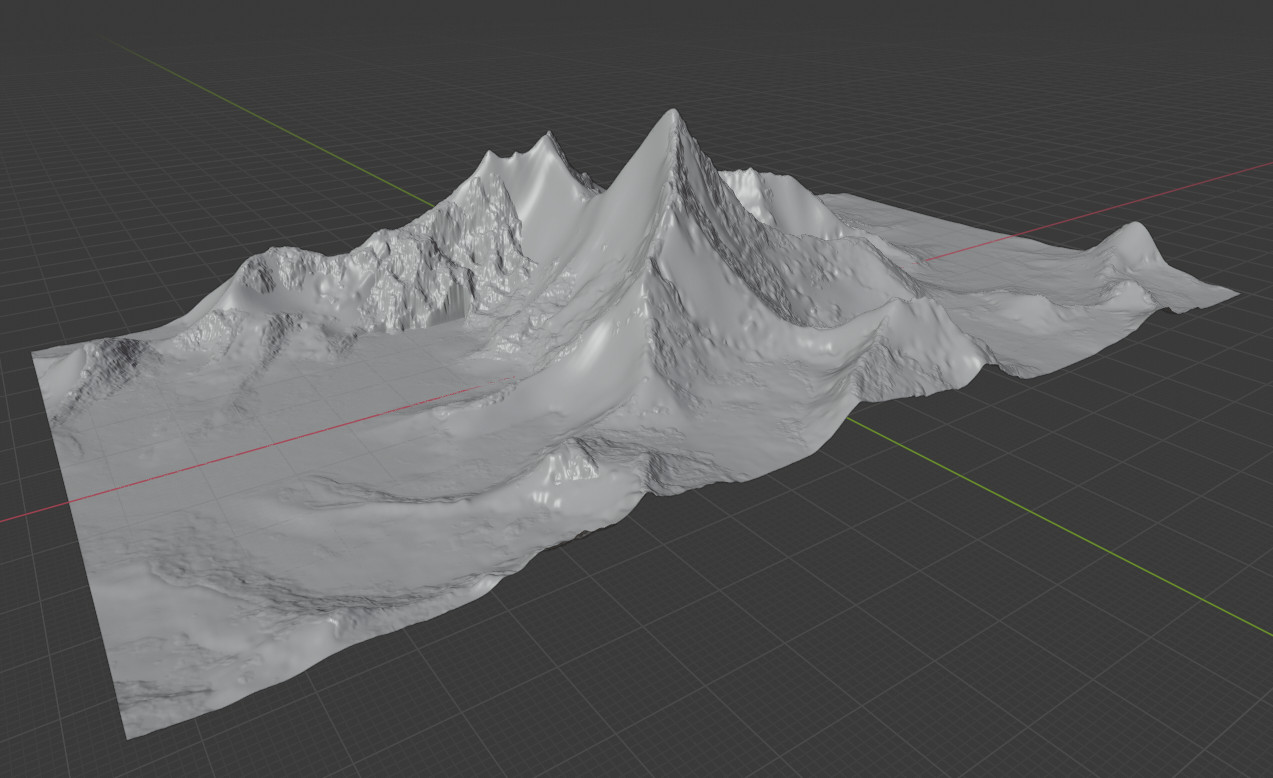
\includegraphics[width=0.95\linewidth]{figures/terrain_everest.jpg}
			\centering
			\caption{Model planinskog vrha Mount Everest u omjeru $1:1$}
			\label{fig:terrain_everest}
		\end{figure}
	
	
	
	\section{Određivanje visine terena u proizvoljnoj točki}
	
		Za potrebe ispravnog postavljanja objekata na teren nužno je poznavanje visine modela terena u bilo kojoj točki.
		Problem je moguće formalizirati kao traženje vrijednosti funkcije $f \colon \mathbb{R}^2 \to \mathbb{R}$ koja iz para koordinata $(x, y)$ određuje vrijednost \mbox{$z$ koordinate}.
		
		\textit{Blender} za to ne nudi gotovo rješenje.
		Međutim, moguće je dohvatiti globalne koordinate svih vrhova u modelu.
		S obzirom na to da je približno rješenje dovoljno dobro, problem se može modificirati tako da se traže vrhovi mreže \engl{mesh} koji su, gledajući jedino projekciju na $xOy$ ravninu, \textit{blizu} tražene točke.
		Vrijednosti njihovih $z$ koordinata tada se mogu koristiti za predviđanje vrijednosti $z$ koordinate u točki $(x,y)$.
		U ovom slučaju \textit{bliskim} vrhovima smatraju se vrhovi iz skupa $V'$ definiranog formulom \ref{eq:close_points}, pri čemu $V$ označava skup svih vrhova modela.
		\begin{equation}
			V' = \{\, v \in V \, \mid \, \left| v.x - x \right| < d \, \land \, \left| v.y - y \right| < d \,\}\label{eq:close_points}
		\end{equation}
		
		Testiranjem različitih vrijednosti parametra $d$ odlučeno je postaviti ga na \SI{70}{\percent} iznosa udaljenosti između susjednih vrhova, odnosno vrijedi $d=$~\SI{2.8}{\meter}.
		
		Vremenski efikasan pronalazak elemenata skupa $V'$ postiže se modificiranim dvodimenzionalnim binarnim pretraživanjem.
		Obavlja se pretprocesiranje podataka u kojem se svi vrhovi grupiraju i sortiraju prema vrijednostima $x$ koordinate.
		Vrhovi u svakoj tako nastaloj grupi potom se sortiraju prema vrijednosti $y$ koordinate.
		Time je omogućeno binarno pretraživanje prvo po $x$ koordinati, a zatim unutar grupe po $y$ koordinati.
		Od standardnog binarnog pretraživanja ovo pretraživanje razlikuje se po tome što u prvom koraku može pronaći više grupa, odnosno u drugom koraku više vrhova.
		S prethodno definiranom vrijednošću parametra $d$, algoritam može vratiti $0$, $1$, $2$ ili $4$ različita vrha.
		
		Za mrežu od $n \times m$ vrhova, dvodimenzionalno binarno pretraživanje, nakon pretprocesiranja, za svaki upit ima složenost $O(\log n + \log m) = O(\log(nm))$, dok trivijalno slijedno pretraživanje cijelog skupa $V$ ima složenost $O(nm)$.
		
		Alternativno rješenje jest indeksiranje vrhova u modelu terena uporabom strukture podataka \textit{R-stablo} koje se često primjenjuje u geografskim informacijskim sustavima (GIS)~\cite{wiki:rtree}.
		Primjeri \textit{Python} biblioteka trećih strana koje implementiraju R-stablo su \mbox{\textit{Rtree}}\footnote{\url{https://rtree.readthedocs.io/}} i \mbox{\textit{GeoPandas}}\footnote{\url{https://geopandas.org/}}.



\chapter{Građevine}
	
	\section{Izvor podataka}
	
		\textit{OpenStreetMap}\footnote{\url{https://www.openstreetmap.org/}} (dalje u tekstu: OSM) pokazao se najboljim izvorom podataka o građevinama za potrebe ovog rada.
		
		Iako za područje grada Zagreba postoje značajno detaljniji podatci od onih koje pruža OSM, poput podataka nastalih višegodišnjim aerofotogrametrijskim i LiDAR snimanjima grada,\footnote{\url{https://zagreb.gdi.net/zg3d/}} dohvaćanje tih podataka nije jednostavno jer se korisnicima ne nudi nikakvo sučelje \engl{Application programming interface -- API}.
		
		S druge strane, uz OSM postoji \textit{Overpass} API i njemu pripadni jezik za pisanje strukturiranih upita \engl{Overpass Query Language} koji korisnicima omogućuje gotovo trivijalno pretraživanje i dohvaćanje podataka dostupnih u OSM bazi~\cite{wiki:overpassapi}\cite{wiki:overpassql}.
		Za \textit{Overpass} API razvijeno je i grafičko web sučelje pod imenom \textit{Overpass Turbo}~\cite{wiki:overpassturbo}.\footnote{\url{https://overpass-turbo.eu/}}
	
	
	
	\section{Struktura \textit{OpenStreetMap} podataka}
	
		Podatci koje \textit{Overpass} API vraća sastoje se od popisa čvorova \engl{node}, puteva \engl{way} i relacija \engl{relation} u JSON (\textit{JavaScript Object Notation})\footnote{\url{https://www.json.org/}} formatu.
		Svaki element ima jedinstveni cjelobrojni identifikator.
		
		Čvorovi imaju podatke o svojoj geografskoj širini i dužini.
		Putevi su definirani listom čvorova.
		Zatvorene petlje posebna su vrsta puteva kojima su prvi i zadnji čvor jednaki te se u pravilu koriste za opisivanje poligona.
		Relacije se sastoje od više puteva koji su najčešće ujedno i zatvorene petlje.
		
		Svi elementi mogu imati dodatne metapodatke (oznake).\footnote{\url{https://wiki.openstreetmap.org/wiki/Tags}}
		Za potrebe dohvaćanja i stvaranja zgrada interesantni su metapodatci koji razlikuju građevine od ostalih OSM podataka, kao i metapodatci o visini pojedine građevine.
		
		U ovom radu zgradama se smatraju svi putevi i relacije koji imaju postavljenu bilo kakvu vrijednost oznaka \texttt{building}\footnote{\url{https://wiki.openstreetmap.org/wiki/Key:building}} ili \texttt{building:part}\footnote{\url{https://wiki.openstreetmap.org/wiki/Key:building:part}} bez njihove daljnje analize~\cite{wiki:simple3d}, te se upravo takav upit šalje prema OSM bazi koristeći \textit{Overpass} API.
		Razlog tome jest što na globalnoj razini više od \SI{81}{\percent} građevina ima jednostavnu oznaku \texttt{building=yes},\footnote{\url{https://taginfo.openstreetmap.org/keys/building#values}} dok više od \SI{86}{\percent} zgrada ima oznaku \texttt{building:part=yes},\footnote{\url{https://taginfo.openstreetmap.org/keys/building:part#values}} bez dodatnog specificiranja tipova zgrada.
		
		Podatci o visini pojedine zgrade dostupni su kroz nekoliko različitih oznaka.
		Standardne su oznake \texttt{height}\footnote{\url{https://wiki.openstreetmap.org/wiki/Key:height}} i \texttt{building:height} kojima se obilježava ukupna visina u metrima.
		Posredni način određivanja visine moguć je koristeći podatak o broju etaža zgrade, zapisan u oznakama \texttt{levels}, \texttt{building:levels}\footnote{\url{https://wiki.openstreetmap.org/wiki/Key:building:levels}} i \texttt{roof:levels}.
		
		Bilo kakvi podatci o visini zgrada u Zagrebu zapravo su vrlo rijetki.
		Od približno \SI{83 000}{} zgrada koje postoje u OSM bazi, njih svega \SI{3.74}{\percent} ima podatke o točnoj visini ili broju etaža.
		Taj odnos vizualiziran je slikom \ref{fig:overpass_zagreb_height_data}.
		Za sve ostale zgrade visina se odabire kao slučajan broj iz uniformne distribucije na intervalu $\left[8, 25\right]$.
		
		\begin{figure}[ht]
			\centering
			\begin{subfigure}{.48\textwidth}
				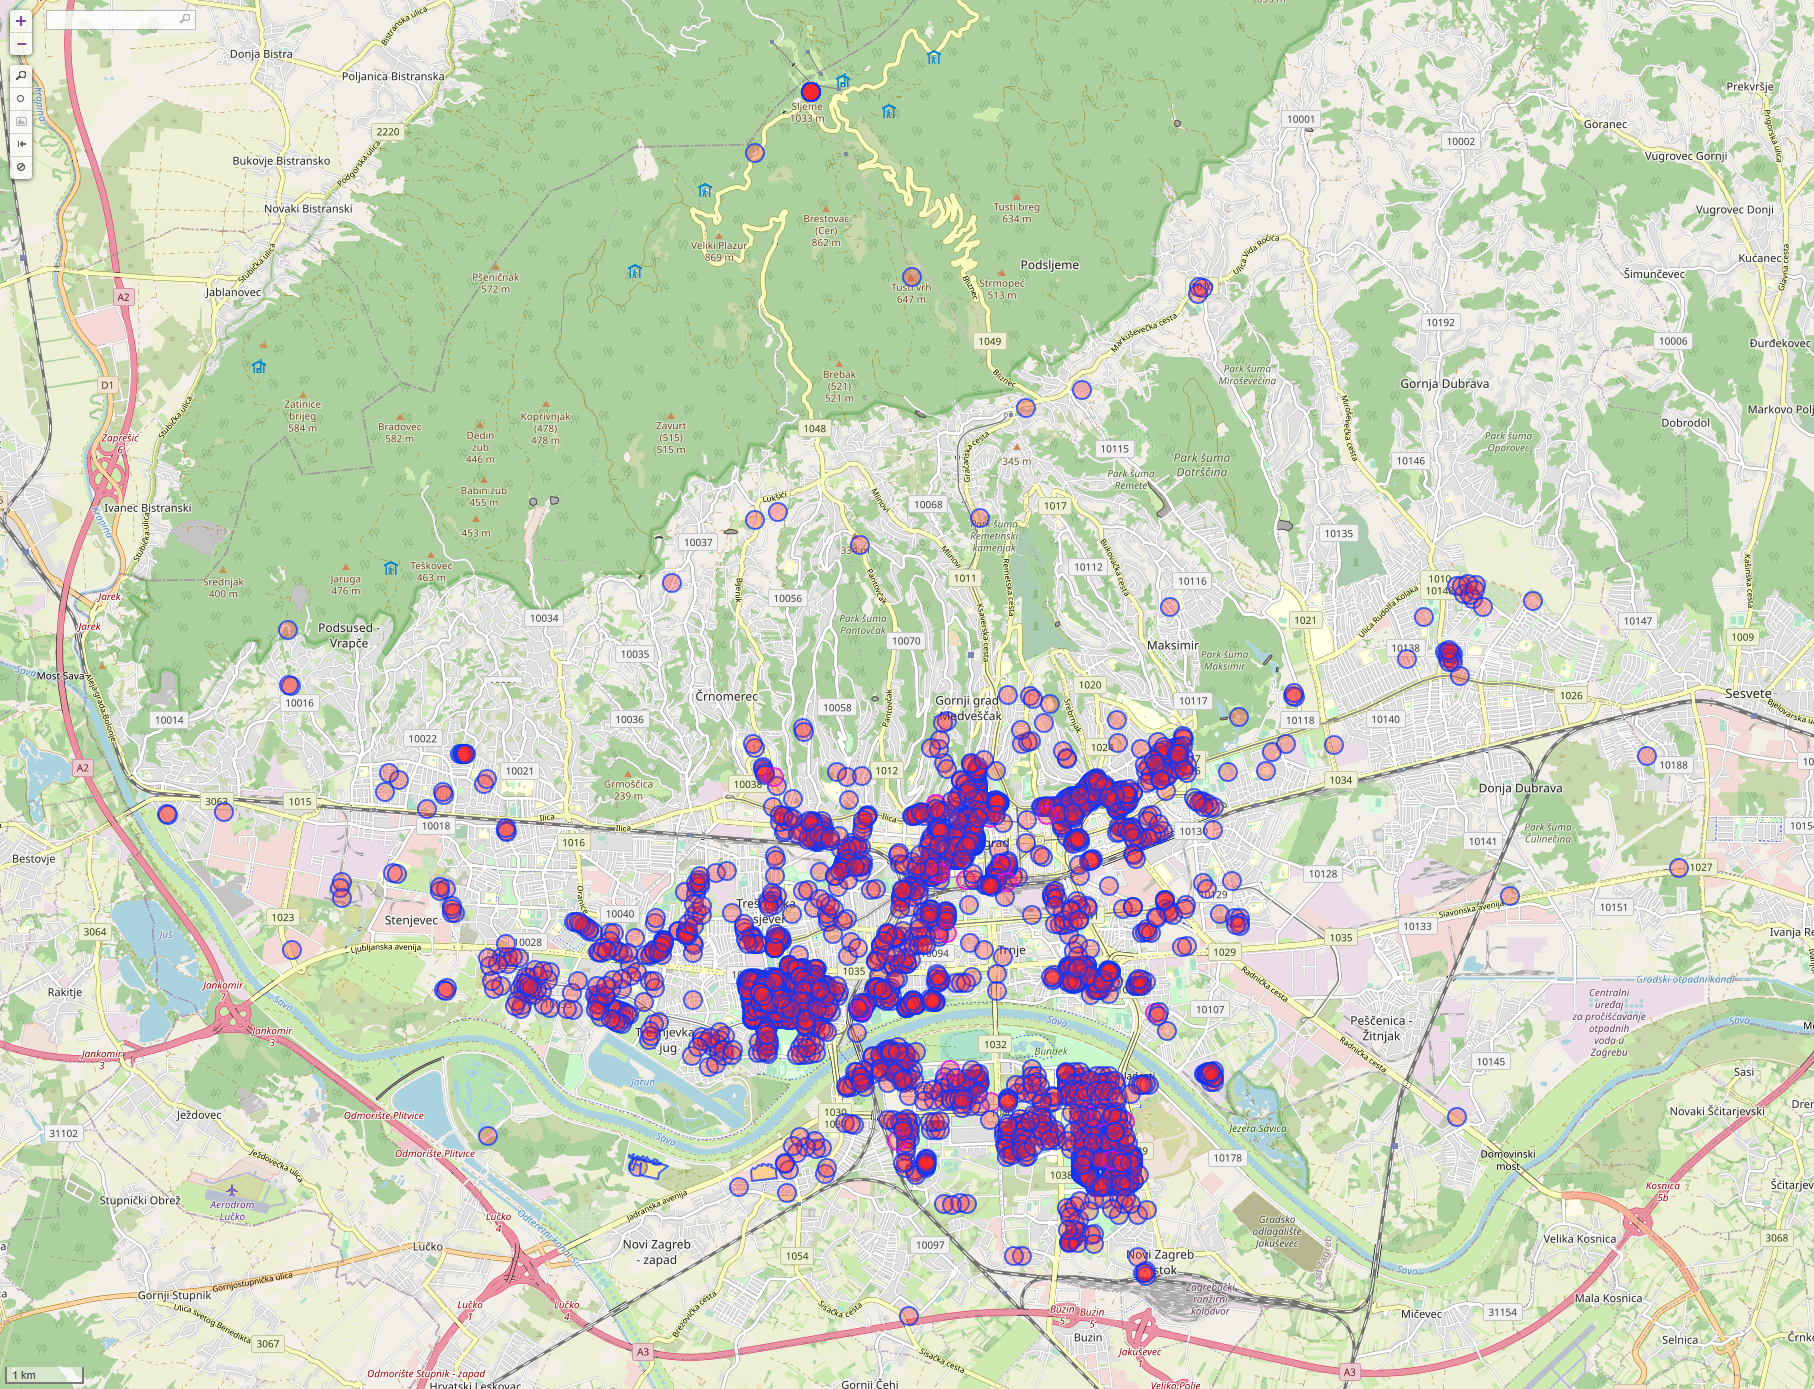
\includegraphics[width=\linewidth,left]{figures/overpass_zagreb_all_buildings_with_height.png}
				\captionsetup{margin=.4cm}
				\caption{Sve građevine u Zagrebu za koje postoje podatci o visini}
				\label{fig:overpass_zagreb_all_buildings_with_height}
			\end{subfigure}
			\hfill
			\begin{subfigure}{.48\textwidth}
				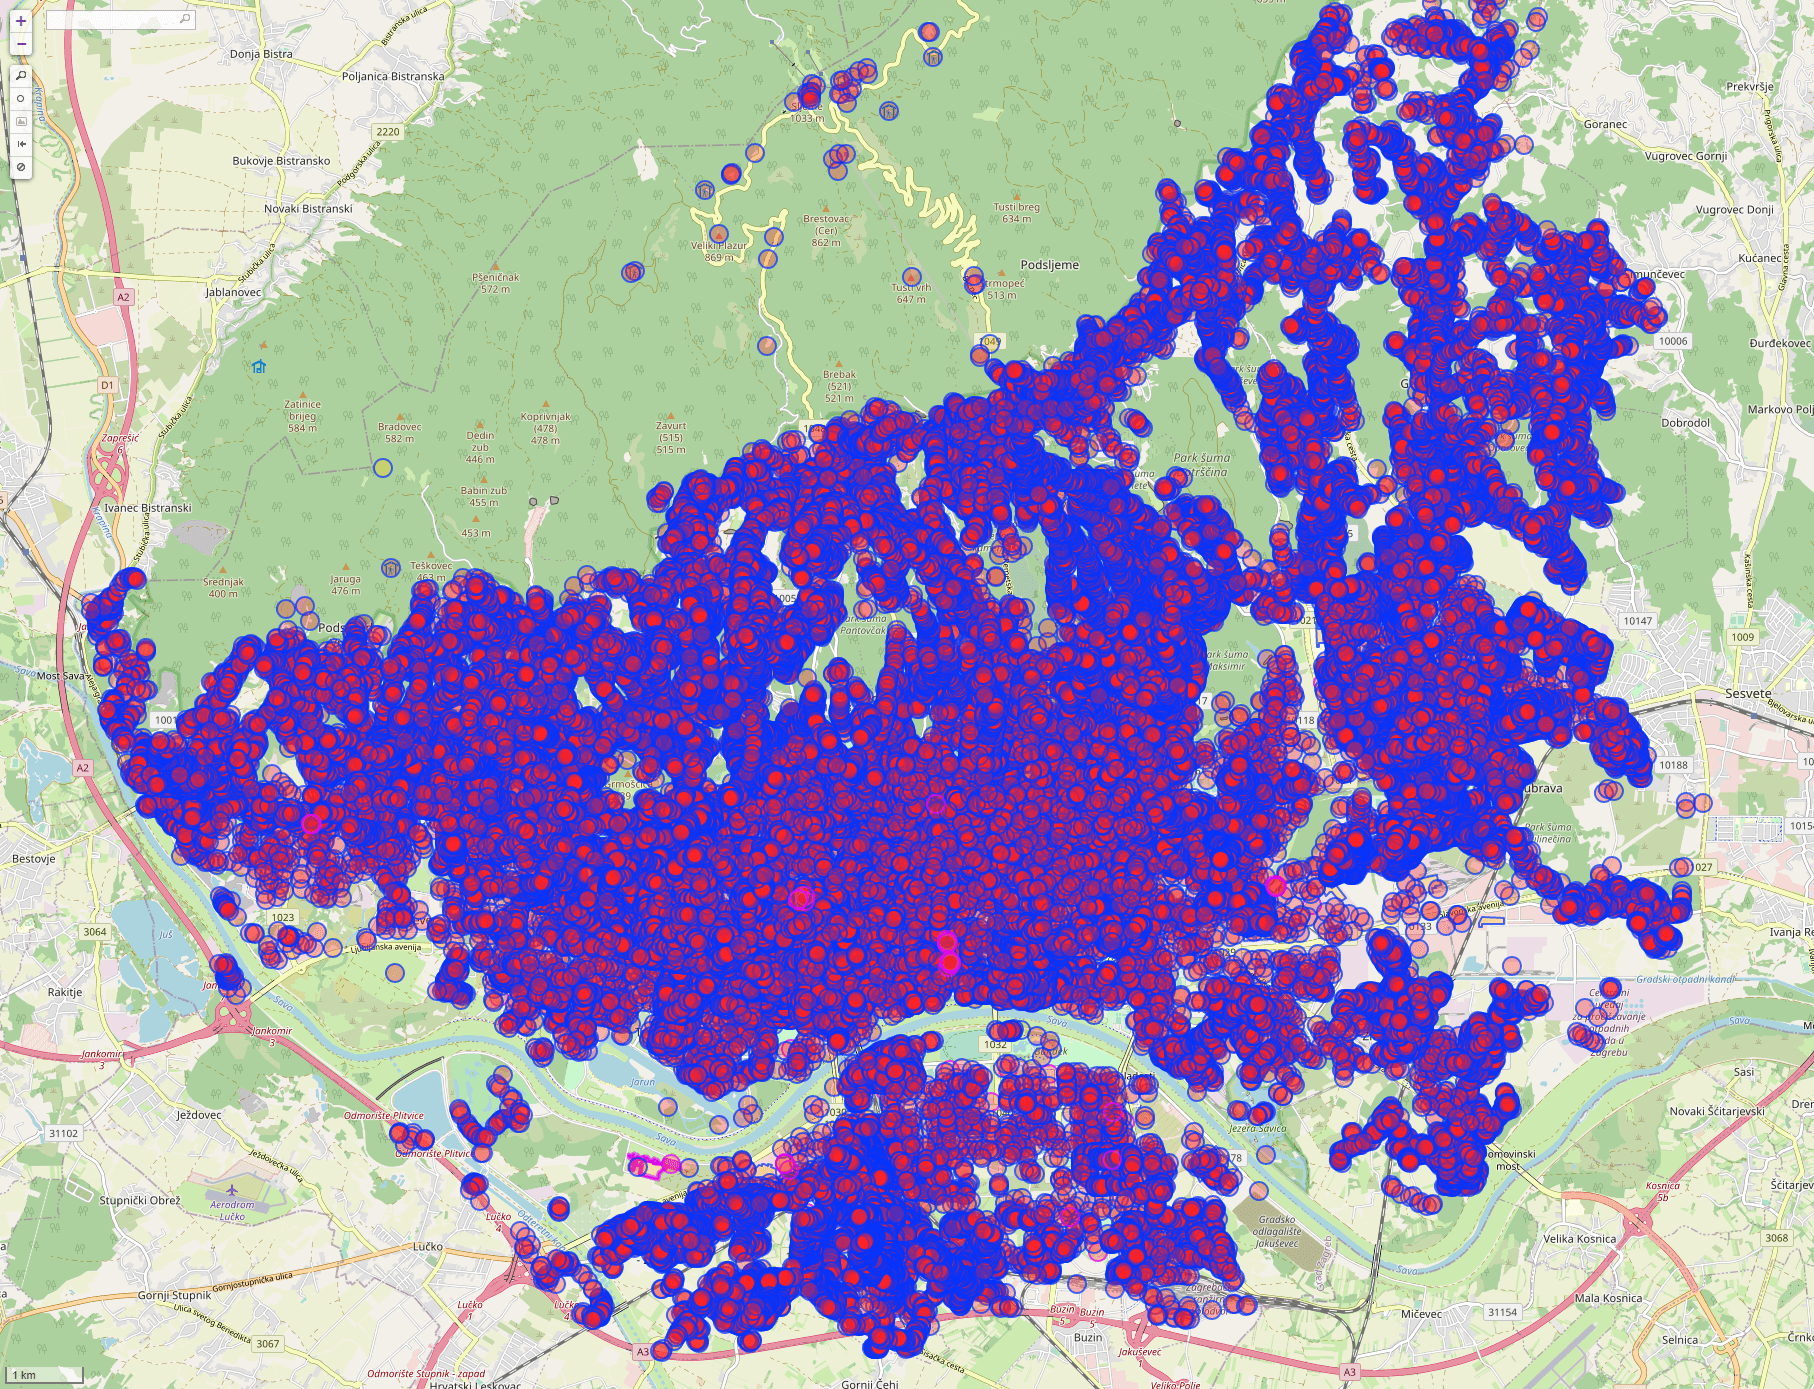
\includegraphics[width=\linewidth,right]{figures/overpass_zagreb_all_buildings.png}
				\captionsetup{margin=.4cm}
				\caption{Sve građevine u Zagrebu, bez postavljenih uvjeta}
				\label{fig:overpass_zagreb_all_buildings}
			\end{subfigure}
			\caption{Vizualizacija OSM podataka o građevinama u Zagrebu (web sučelje \textit{Overpass Turbo})}
			\label{fig:overpass_zagreb_height_data}
		\end{figure}
	
	
	
	\section{Stvaranje 3D modela jednostavnih zgrada}
	
		Jedine informacije na temelju kojih se stvara model zgrade su oblik baze \engl{footprint} i visina zgrade.
		Modeli jednostavnih zgrada, čija se baza sastoji samo od jedne zatvorene petlje, imaju ravne krovove i oblika su prizme.
		
		Za stvaranje mreže \engl{mesh} objekta \textit{Blender} treba dva podatka: listu koordinata vrhova \engl{vertex} i listu stranica \engl{faces}.
		Pri tome je svaka stranica predstavljena listom indeksa vrhova.
		
		Algoritam stvaranja 3D modela zgrade započinje stvaranjem kopije svih $n$ vrhova baze te njihovom translacijom u smjeru pozitivne \mbox{$z$-osi} za iznos visine zgrade čime se dobiva konačna lista od $2n$ vrhova.
		Na slici \ref{fig:mesh_generation} prikazan je model s bazom od $n=6$ vrhova.
		
		Jednostavnim algoritmom, čiji se programski kôd nalazi u isječku \ref{lst:generatefaces}, stvaraju se stranice objekta.
		Prvo se u petlji stvara $n$ bočnih stranica, od kojih svaka ima po dva vrha iz donje baze i dva vrha iz gornje baze.
		Naknadno se dodaju same baze: prvo donja baza s indeksima vrhova u padajućem poretku, a nakon toga gornja baza s indeksima u rastućem poretku.
		Time je stvorena lista svih $n+2$ stranica potrebnih za stvaranje prizme.
	
		\begin{lstlisting}[caption={Isječak programskog kôda za stvaranje stranica 3D modela zgrade},label={lst:generatefaces},frame=L]
def _generate_faces_indices(n: int) -> List[List[int]]:
    faces = [[i, (i + 1) % n, n + (i + 1) % n, n + i]
             for i in range(n)]
    faces.append(list(range(n - 1, -1, -1)))
    faces.append(list(range(n, 2 * n)))
    return faces
		\end{lstlisting}
		
		\begin{figure}[h]
			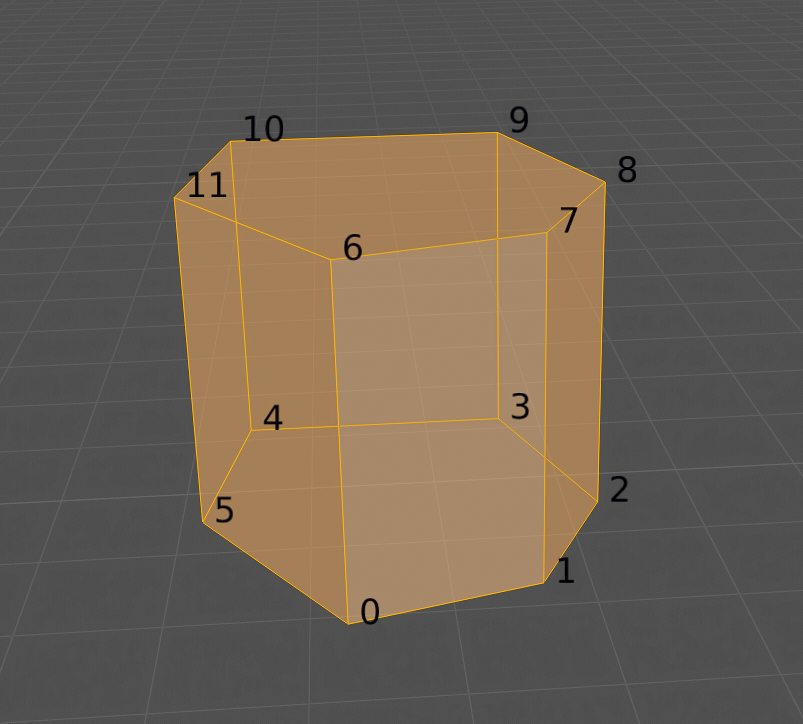
\includegraphics[width=11cm]{figures/mesh_generation.png}
			\centering
			\captionsetup{margin=2cm}
			\caption{Primjer objekta stvorenog iz točaka baze algoritmom \ref{lst:generatefaces}. Vrhovi su obilježeni svojim indeksima.}
			\label{fig:mesh_generation}
		\end{figure}
		
		Ovisno o tome jesu li vrhovi baze zadani u smjeru kazaljke na satu \engl{clockwise -- CW} ili suprotno od smjera kazaljke na satu \engl{counterclockwise -- CCW}, normale svih stranica bit će usmjerene ili prema unutrašnjosti modela ili prema van.
		Radi poštivanja konvencija nad svakim se generiranim objektom poziva naknadno  izračunavanje normala \engl{recalculate normals} ugrađeno u \textit{Blender} tako da su u konačnici sve normale ujednačene i pokazuju iz objekta prema van bez obzira na originalan poredak točaka u bazi.
	
	\eject
	
	
	\section{Stvaranje 3D modela složenih zgrada}
	
		Složenim se zgradama obris sastoji od više poligona \engl{relation}.
		
		Zgrade sastavljene od više susjednih dijelova koji se međusobno ne preklapaju trivijalno se svode na modeliranje jednostavnih zgrada koje je opisano u prethodnom poglavlju -- za svaki dio zgrade \engl{way} u relaciji stvara se po jedna samostalna jednostavna zgrada.
		
		Zgrade čiji je obris u obliku poligona koji u unutrašnjosti ima jednu ili više praznina značajno su teže za modeliranje.
		Njihov model nije prizma u užem smislu riječi.
		Stvaranje takvih objekata obavljeno je konstruktivnom geometrijom čvrstih tijela \engl{Constructive Solid Geometry -- CSG}~\cite{pandzic:virtualna}.
		Prvo se stvara jednostavna zgrada koja je opisana vanjskim poligonom.
		Za svaki unutrašnji poligon koji opisuje jednu prazninu također se stvara po jedna jednostavna zgrada, ali takve su zgrade privremene.
		Koristeći \textit{Blenderov} ugrađeni modifikator za CSG \engl{boolean modifier} sve privremene zgrade oduzimaju se od početne te se potom svi privremeni objekti uklanjaju iz scene.
		Time se dobiva konačni model zgrade kao jedna mreža \engl{mesh}.
		
		Primjer na slici \ref{fig:relations_upper_town} prikazuje složene zgrade u dijelu Gornjeg Grada oko Trga svetoga Marka.
		U gornjem lijevom kutu vidljivi su Banski dvori, dok se u gornjem desnom kutu nalazi Saborska palača.
		U generiranom modelu prikazanom na slici \ref{fig:relations_upper_town_render} naknadno su ručno uklonjene sve jednostavne zgrade.
	
		\begin{figure}[h]
			\centering
			\begin{subfigure}{.5\textwidth}
				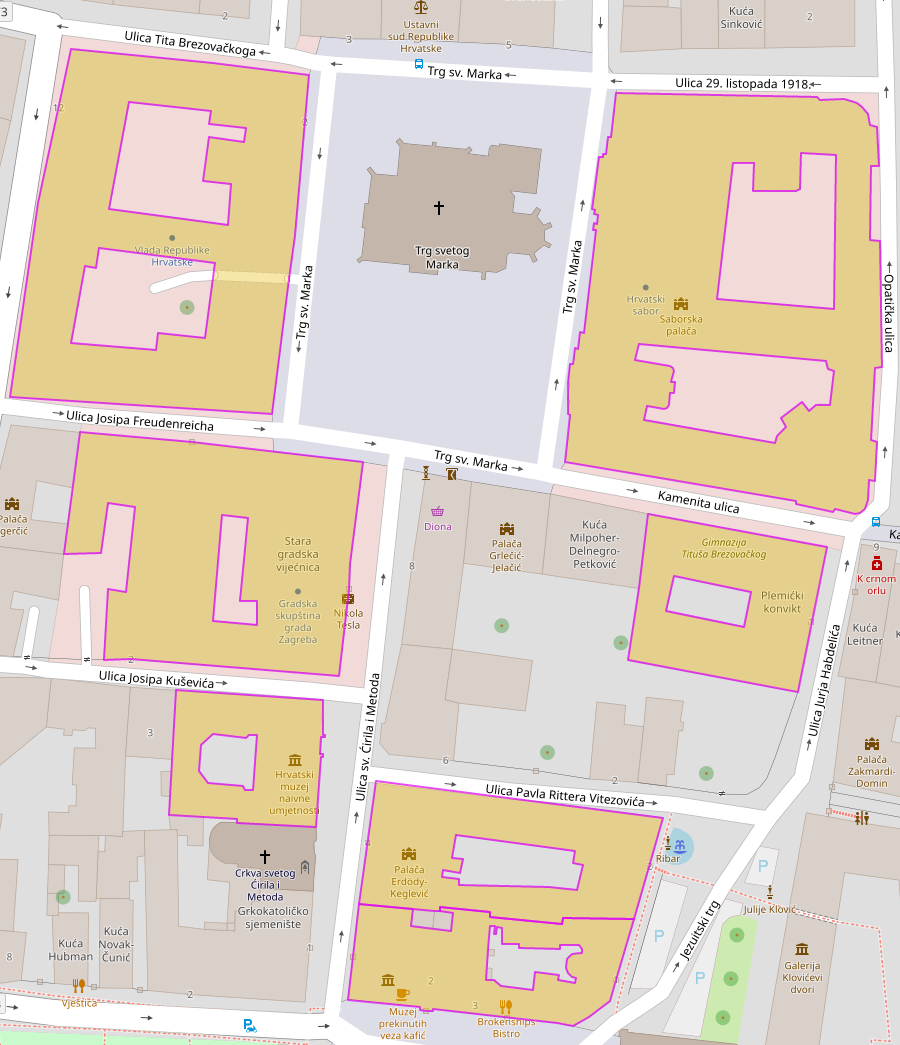
\includegraphics[width=.975\linewidth,left]{figures/relations_upper_town_map.png}
				\caption{Slika iz web sučelja \textit{Overpass Turbo}}
				\label{fig:relations_upper_town_map}
			\end{subfigure}%
			\begin{subfigure}{.5\textwidth}
				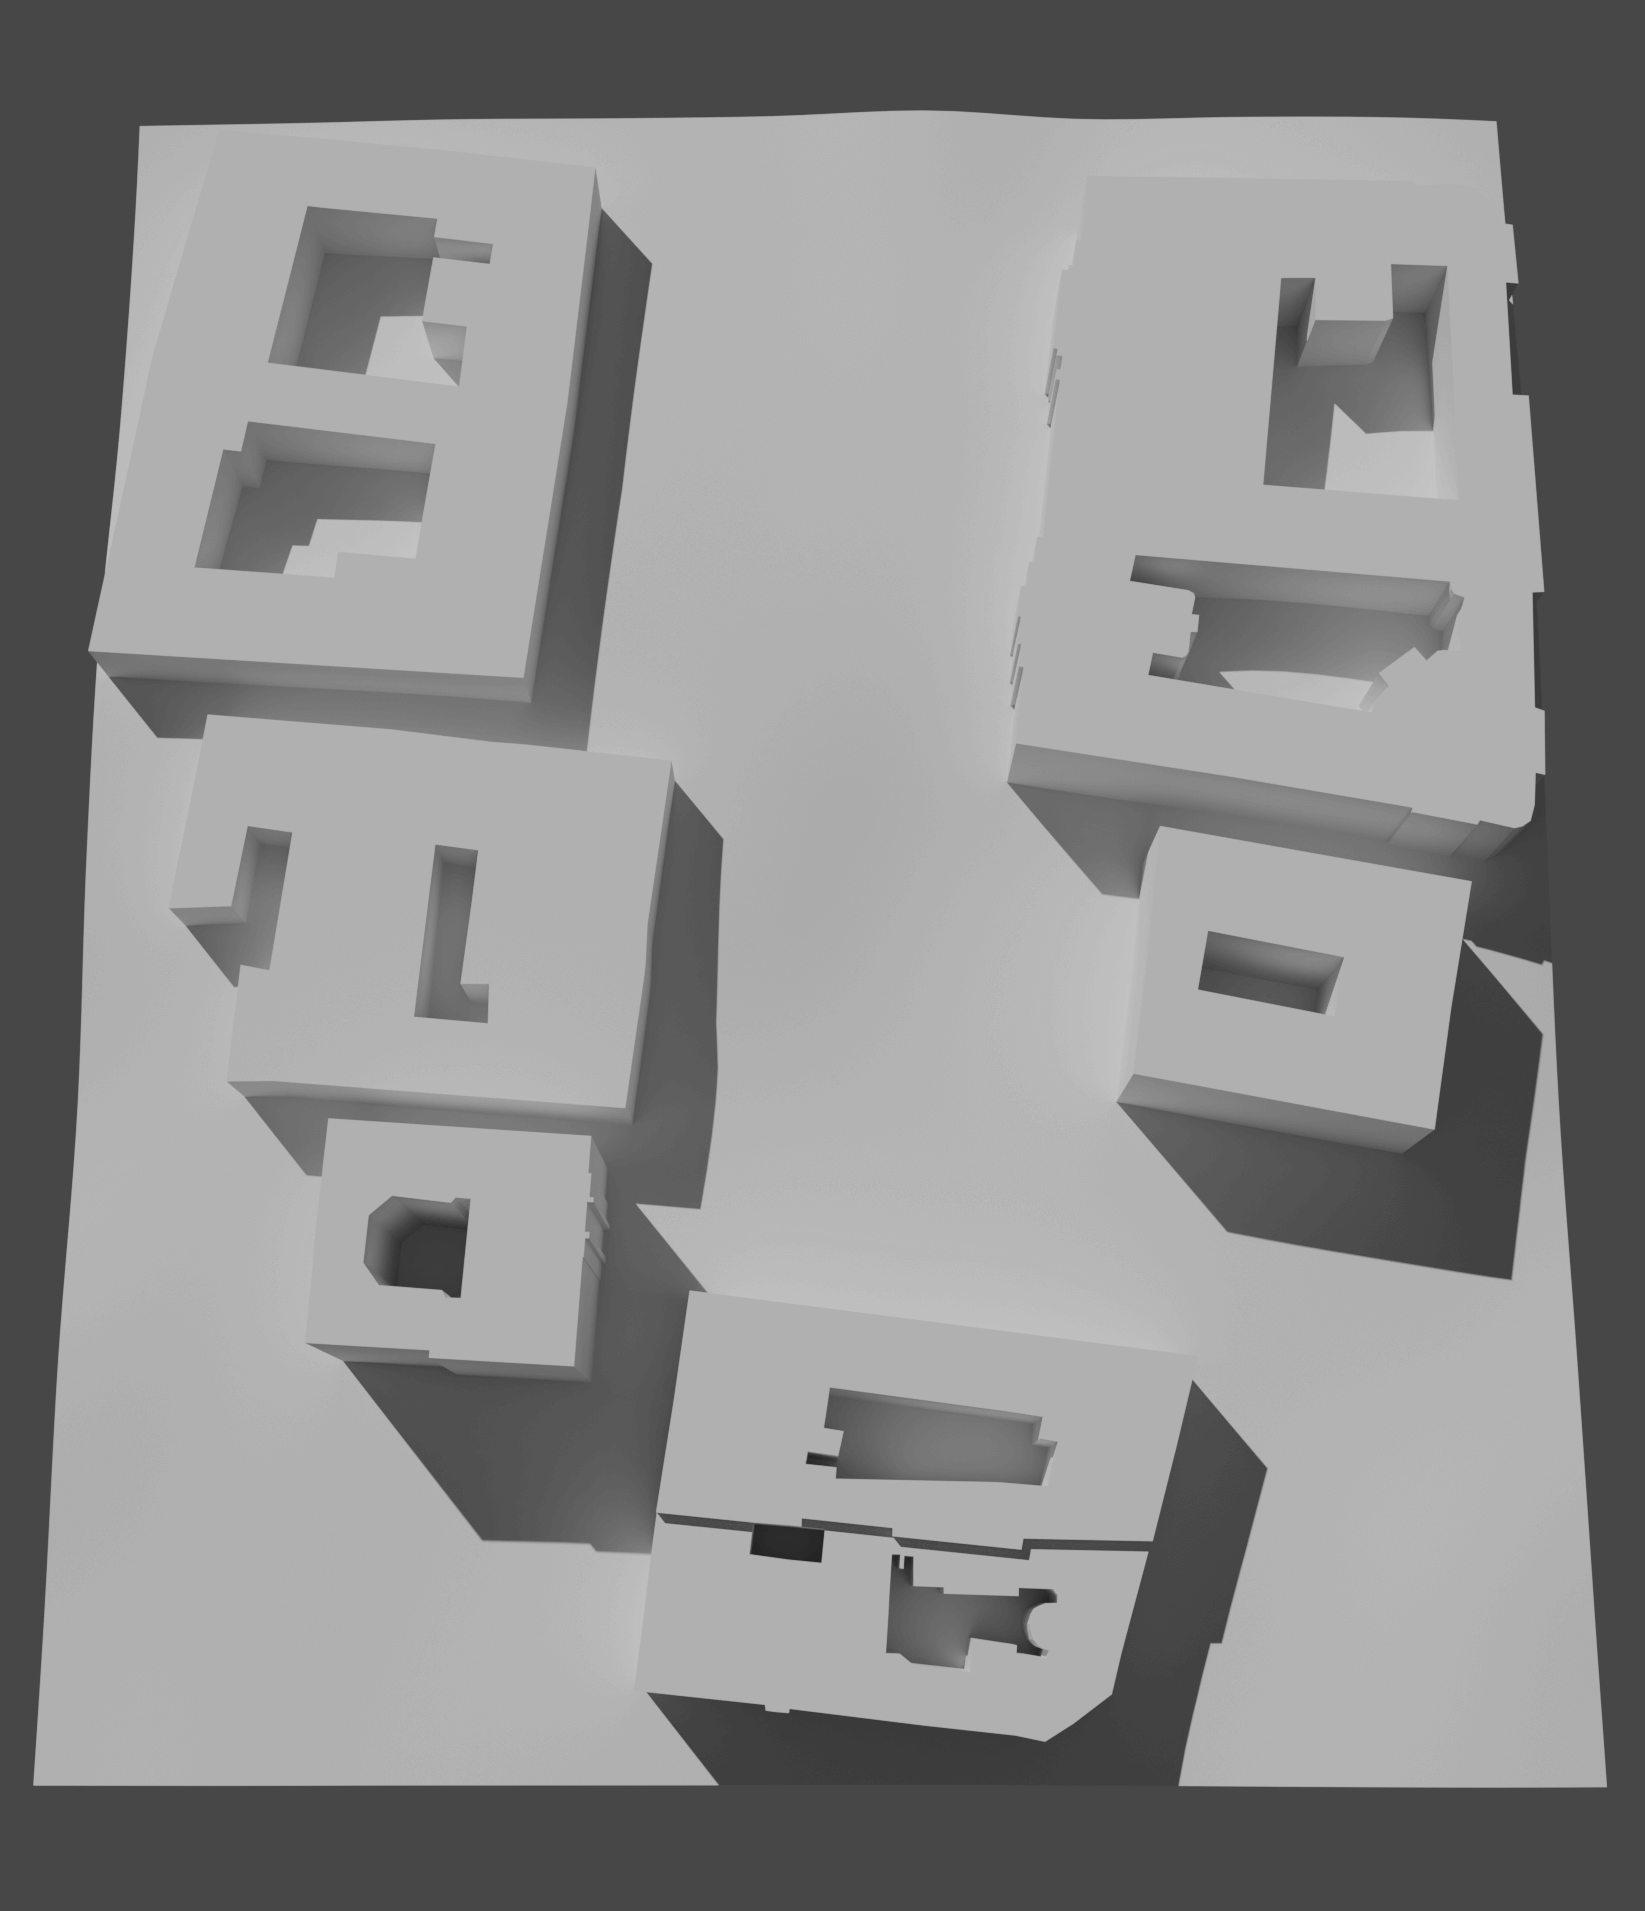
\includegraphics[width=.975\linewidth,right]{figures/relations_upper_town_render.png}
				\caption{Generirani model dijela grada}
				\label{fig:relations_upper_town_render}
			\end{subfigure}
			\caption{Složene zgrade na Gornjem Gradu (Trg svetoga Marka)}
			\label{fig:relations_upper_town}
		\end{figure}
	
	
	
	\section{Uređivanje javno dostupnih podataka}
	
		Podatke koji se pohranjuju u OSM bazi prikupljaju dobrovoljci širom svijeta.
		Bilo tko može kreirati korisnički račun te doprinijeti dodavanjem novih ili ispravljanjem postojećih podataka.
		U svibnju 2020. godine OSM je imao više od $6.5$ milijuna registriranih korisnika.\footnote{\url{https://web.archive.org/web/20200524000234/https://www.openstreetmap.org/stats/data_stats.html}}
		
		Na početku izrade ovog rada o zgradama Fakulteta elektrotehnike i računarstva u OSM bazi je, osim obrisa zgrada, postojalo vrlo malo dodatnih informacija.
		Za potrebe ovog rada podatci su dopunjeni:
		
		\begin{itemize}
			\item visina zgrade C postavljena je na \SI{50}{\meter} (oznaka \texttt{height})~\cite{wiki:zagrebneboderi},
			\item broj etaža zgrade C postavljen je na $13$ (oznaka \texttt{building:levels}),
			\item broj etaža zgrade B postavljen je na $2$,
			\item broj etaža zgrade A postavljen je na $4$,
			\item broj etaža zgrade D postavljen je na $4$,
			\item visina svih šest hodnika koji spajaju zgrade postavljena je na \SI{4}{\meter},
			\item broj etaža svih hodnika postavljen je na $1$,
			\item označeno je da su svi hodnici izrađeni od stakla (oznaka \texttt{building:material}),
			\item svim zgradama i hodnicima oznaka \texttt{building:part} postavljena je na \texttt{university} (prethodne vrijednosti bile su \texttt{yes} ili \texttt{school}).
		\end{itemize}
		
		Osim kroz specijalizirane programe, ažuriranje podataka može se obaviti i u web-pregledniku po izboru.
		Primjer uređivanja podataka vezanih uz zgradu C prikazan je na slici \ref{fig:OSM_edit_C_building}.
		
		\begin{figure}[h]
			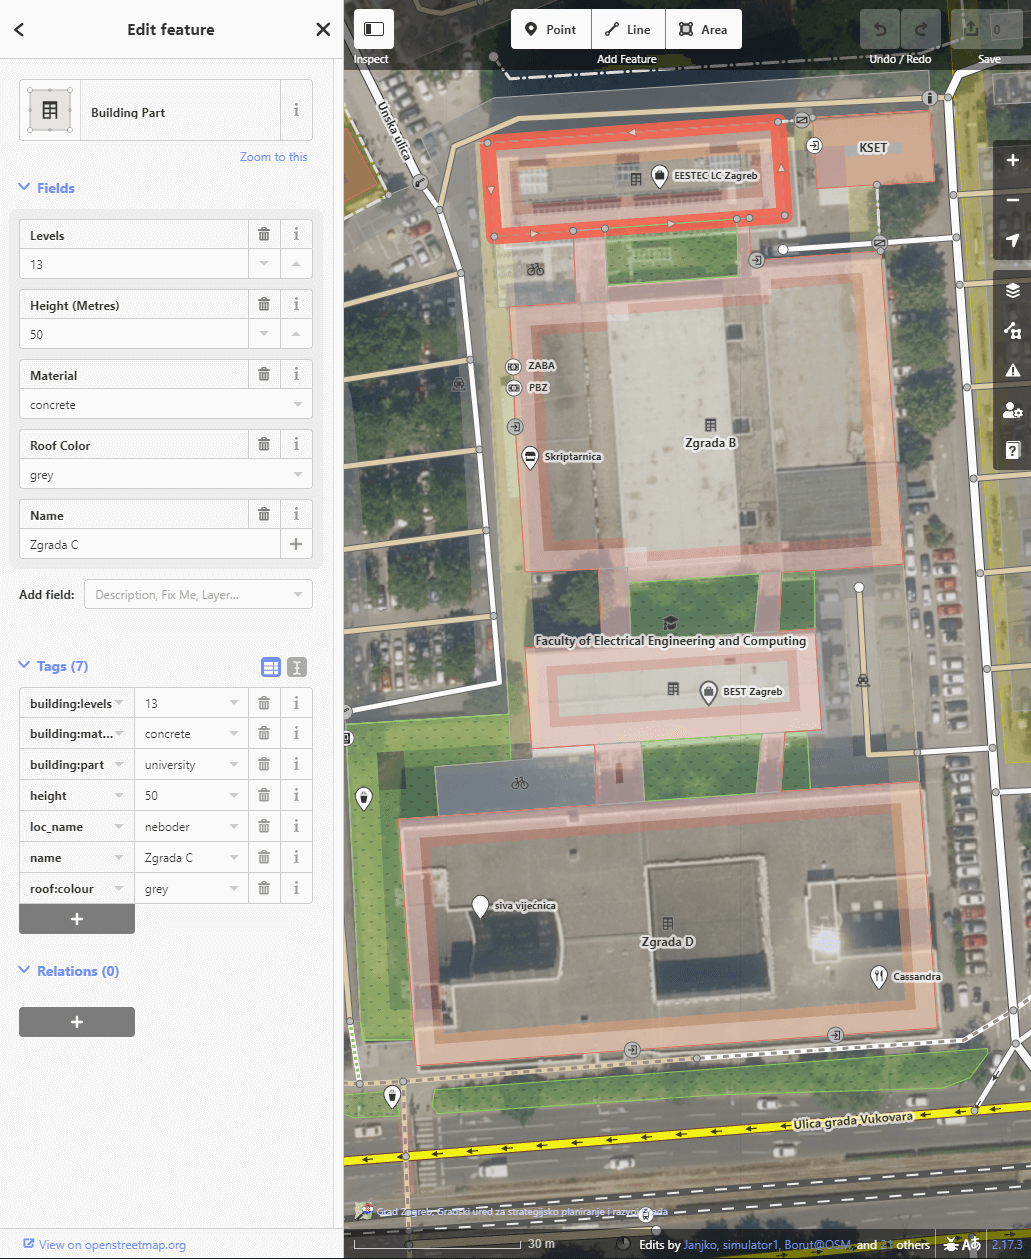
\includegraphics[width=14cm]{figures/OSM_edit_C_building.png}
			\centering
			\caption{Uređivanje OSM podataka o FER-ovoj zgradi C}
			\label{fig:OSM_edit_C_building}
		\end{figure}



\chapter{Stabla}
	
	\section{Izvor podataka}
	
		Najdetaljniji izvor podataka o stablima na području Zagreba jest Katastar zelenila\footnote{\url{https://gis.zrinjevac.hr/}} Zrinjevca\footnote{Podružnica tvrtke Zagrebački Holding d.o.o.}.
		Katastar sadrži lokaciju i druge informacije o svim stablima za čije je održavanje zadužen Zrinjevac te omogućuje jednostavan dohvat podataka na odabranom području u JSON formatu.
		
		Za razliku od koordinatnog sustava EPSG:4326\footnote{\url{https://epsg.io/4326}} koji se koristi u ostatku programskog rješenja i koji točke identificira preko geografske širine i dužine, Katastar sve koordinate vraća u projekcijskom koordinatnom sustavu EPSG:3857 (WGS 84 / Pseudo-Mercator)\footnote{\url{https://epsg.io/3857}}.
		Stoga se sve dohvaćene koordinate prvo moraju transformirati u EPSG:4326 sustav za što se koristi biblioteka \textit{pyproj} odnosno njezin razred \texttt{Transformer}.
	
	
	
	\section{Modeli stabala}
	
		U generiranom modelu grada koriste se tri vrste stabala čiji su primjerci prikazani na slici \ref{fig:tree_types}.
		Vrsta stabla na pojedinoj lokaciji bira se nasumično.
		
		Deblo svakog stabla predstavljeno je krnjim stošcem.
		Krošnje su predstavljene s tri različita objekta:
		\begin{itemize}
			\item stožac s varijabilnim brojem vrhova baze, polumjerom baze i visinom,
			\item geodetska sfera \engl{Ico Sphere}\footnote{Sfera sastavljena od trokuta.} s varijabilnim polumjerom,
			\item UV sfera \engl{UV Sphere}\footnote{Sfera sastavljena od četverokuta.} s varijabilnim brojem prstena, segmenata i \mbox{polumjerom}.
		\end{itemize}
		
		Svi opisani parametri slučajno se biraju iz uniformnih distribucija.
		Radi smanjenja broja vrhova i poligona u modelu grada koji može imati i desetak tisuća stabala većinom se koriste stošci i sfere s malim brojem vrhova.
		
		\begin{figure}
			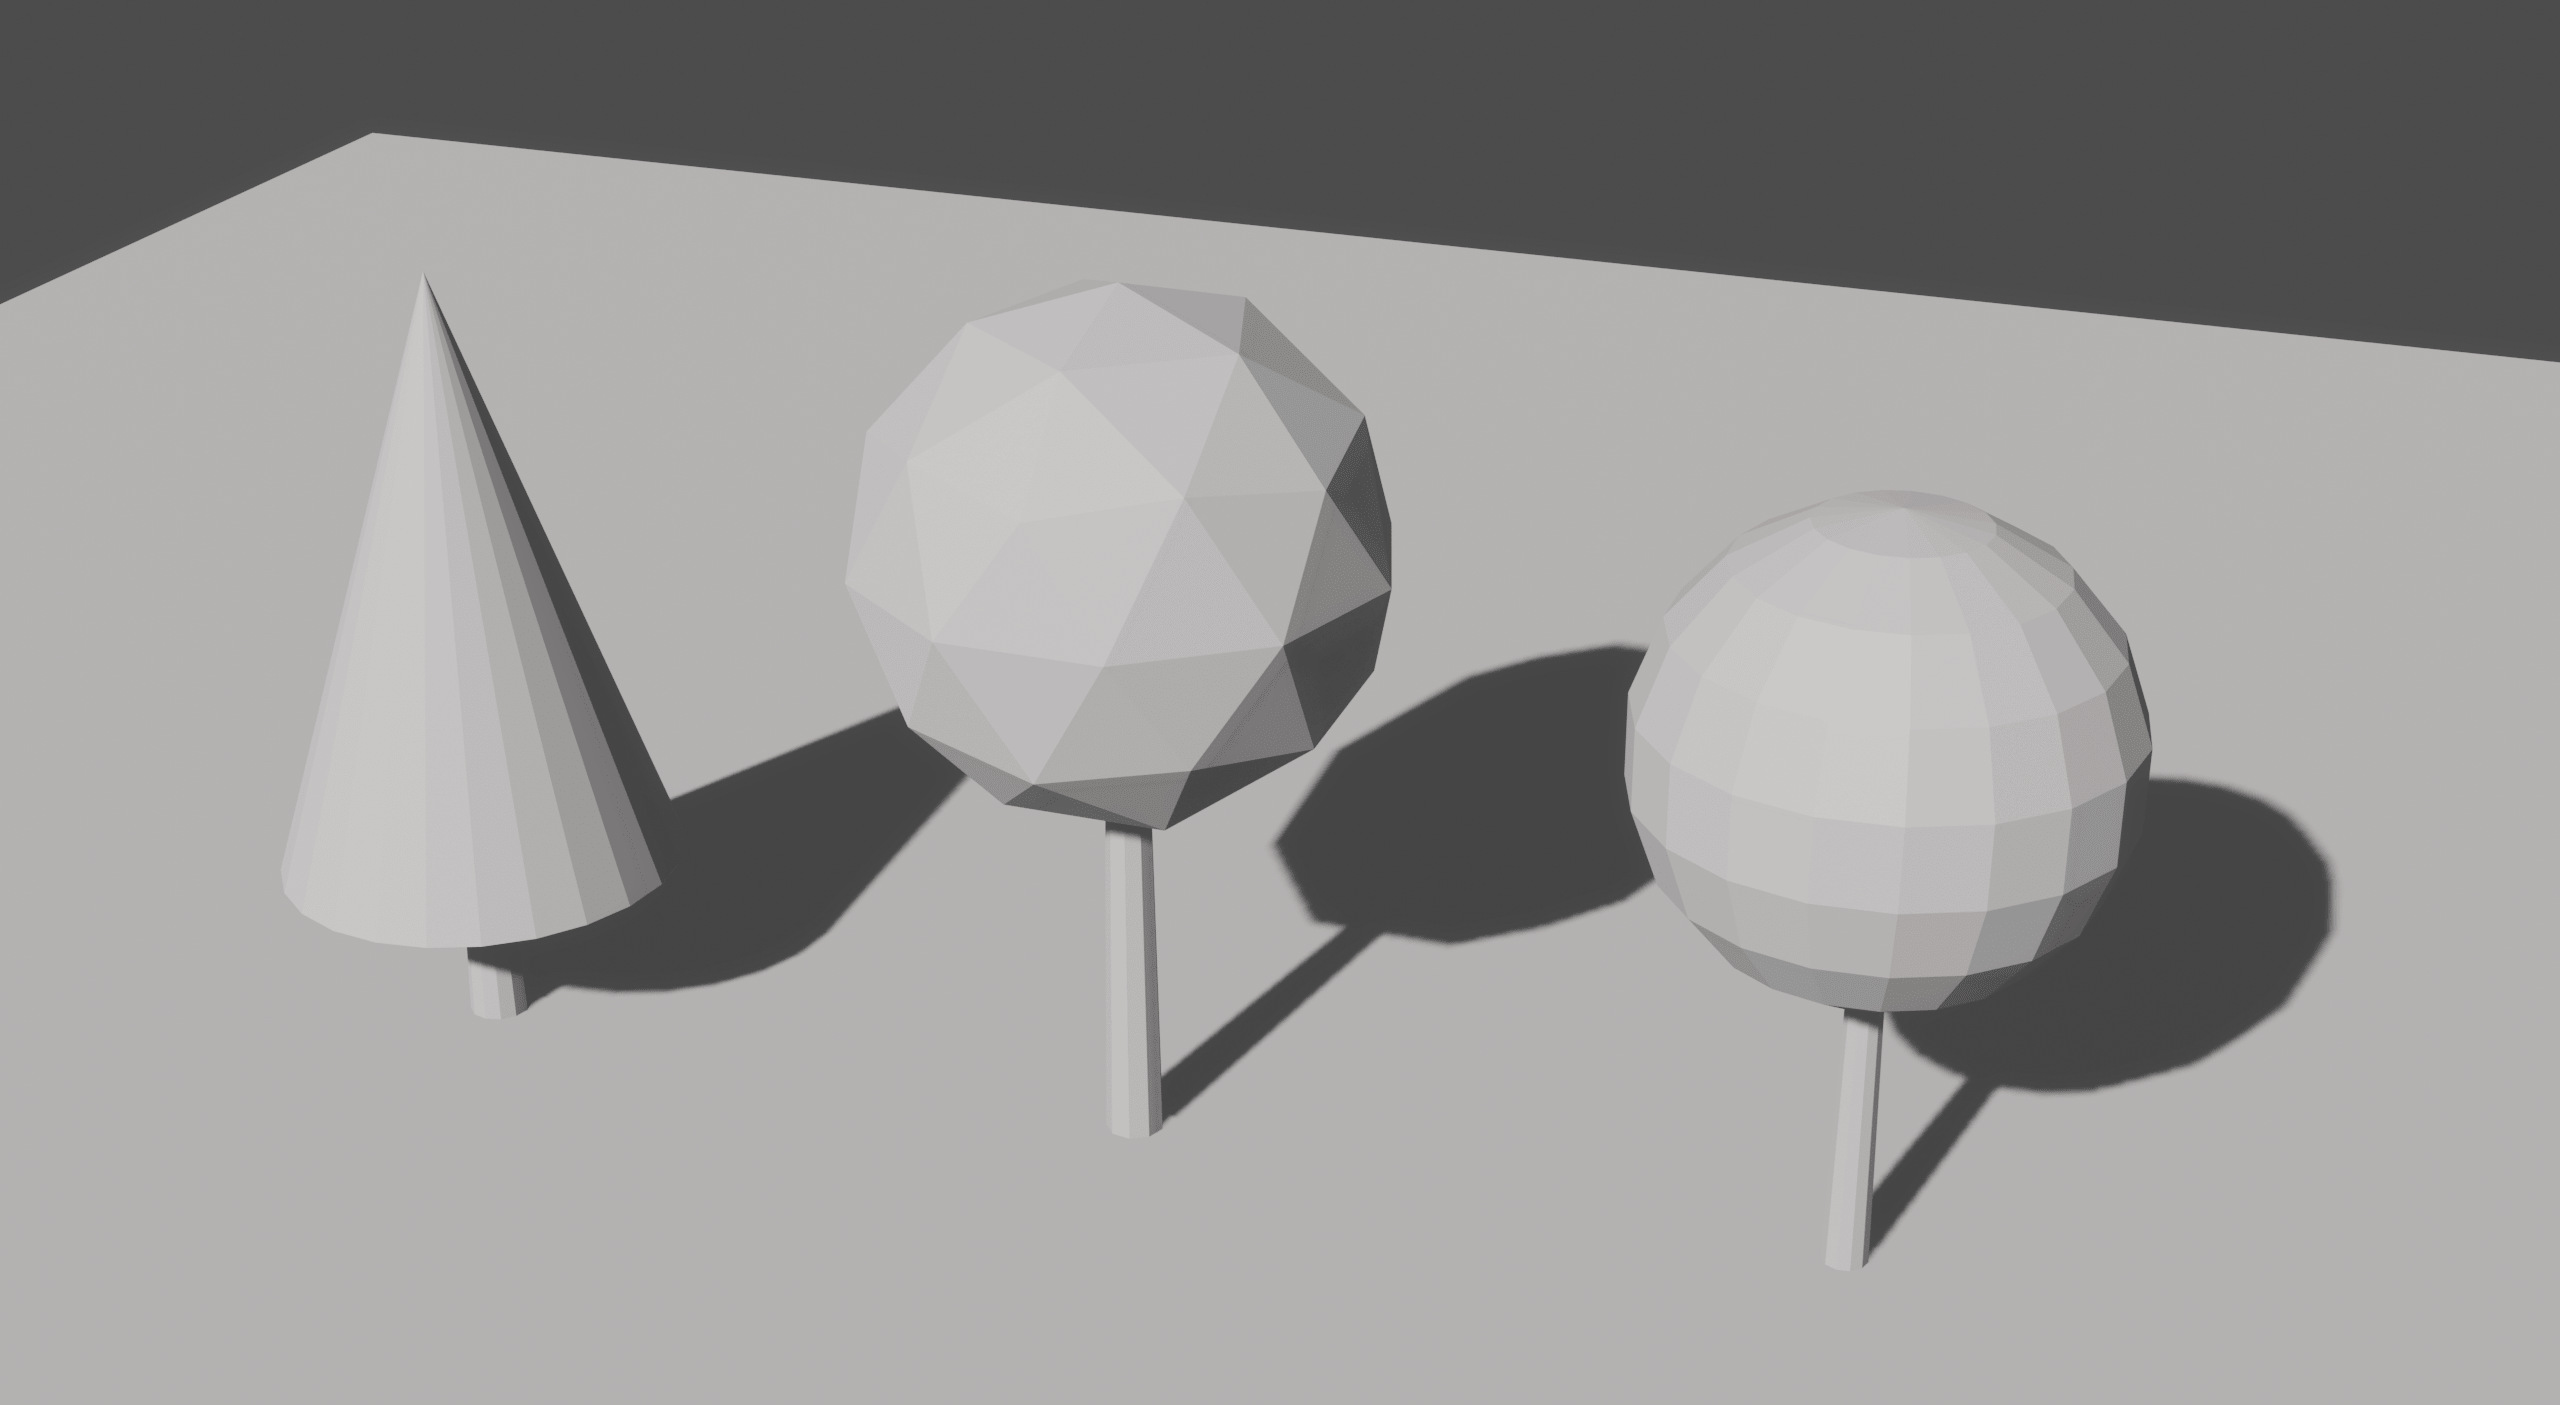
\includegraphics[width=.9\linewidth]{figures/tree_types.jpg}
			\centering
			\caption{Tri vrste stabala koja se koriste u modelu grada}
			\label{fig:tree_types}
		\end{figure}



\chapter{Rezultati}
	
	Razvijeni \textit{Blender} dodatak kao rezultat izvođenja u scenu dodaje sve generirane objekte -- teren, zgrade i drveće.
	Oni se dalje mogu po potrebi ručno uređivati.
	Stvoreni su objekti jednostavni i sastoje se samo od mreže vrhova bez tekstura ili drugih posebnih podataka.
	
	Na slici \ref{fig:fer_basic_render} vidljiv je izrađeni prikaz \engl{render} zgrada Fakulteta elektrotehnike i računarstva kao i sportske dvorane Martinovka i okolnih zgrada.
	Nakon uređivanja OSM podataka sve zgrade i hodnici ispravnih su dimenzija.
	
	\begin{figure}[H]
		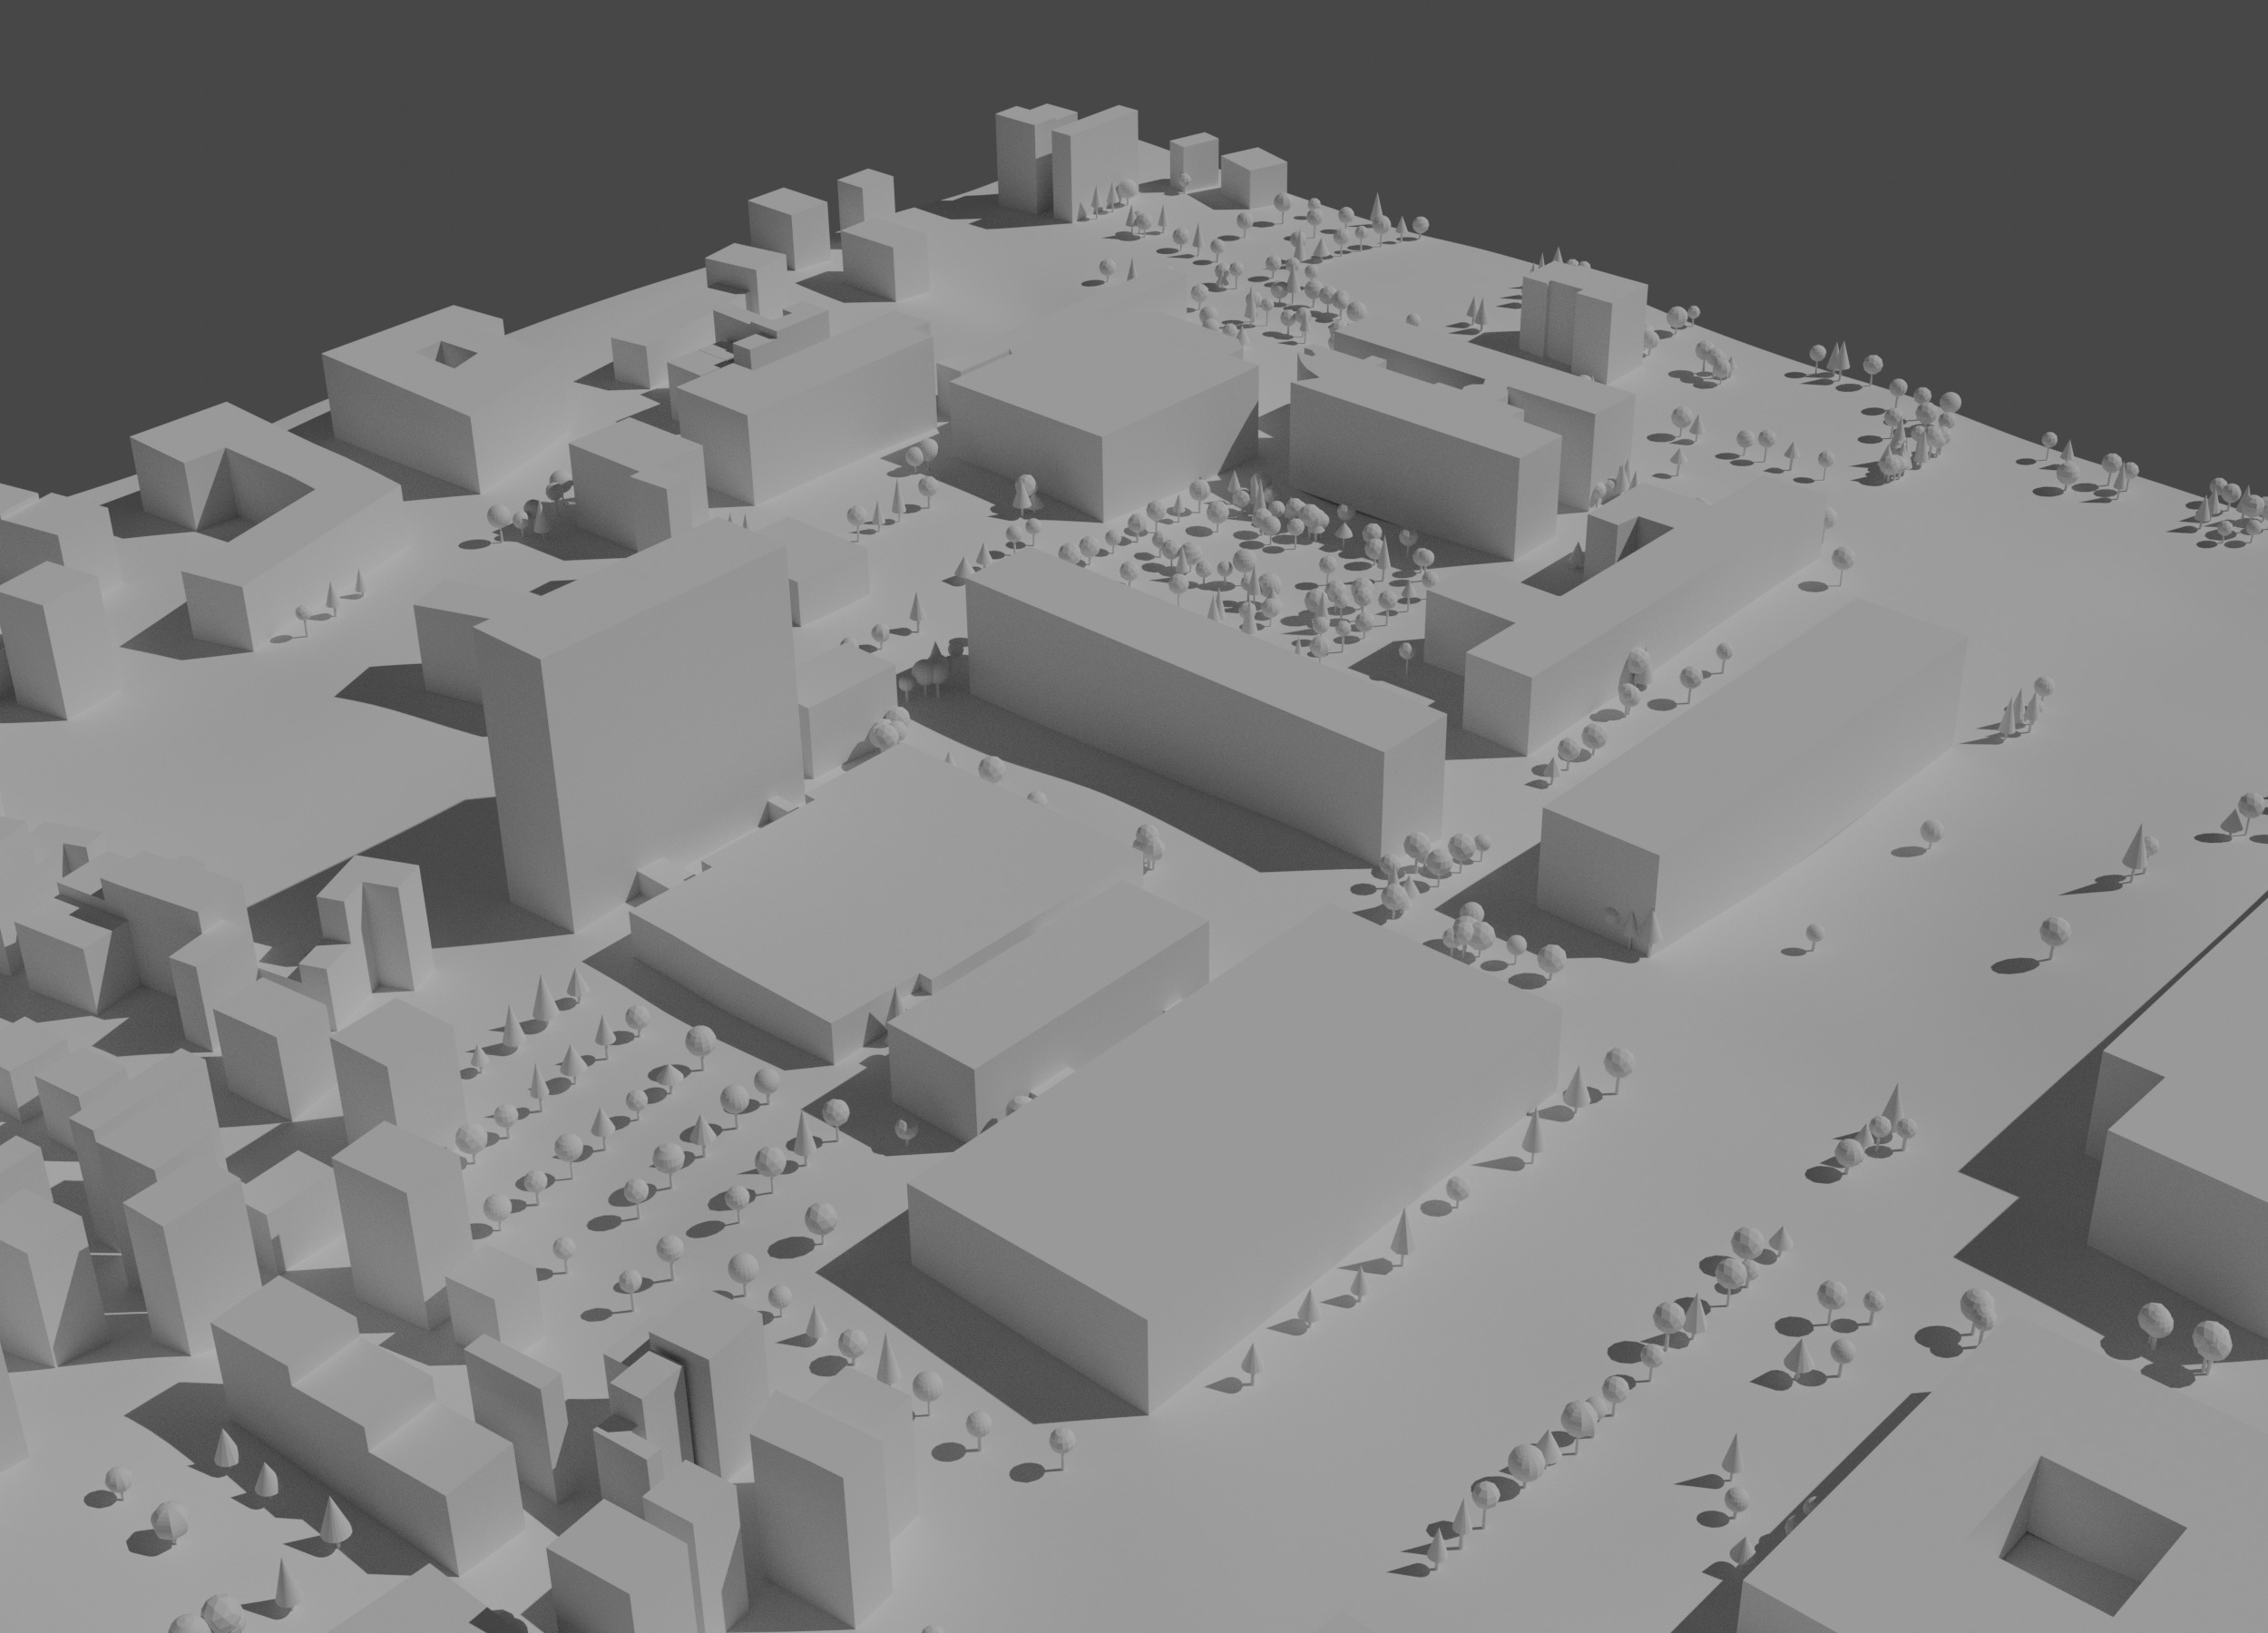
\includegraphics[width=\linewidth]{figures/fer_basic_render.jpg}
		\centering
		\caption{Model zgrada Fakulteta elektrotehnike i računarstva}
		\label{fig:fer_basic_render}
	\end{figure}
	
	\begin{figure}[H]
		\centering
		\begin{subfigure}{\linewidth}
			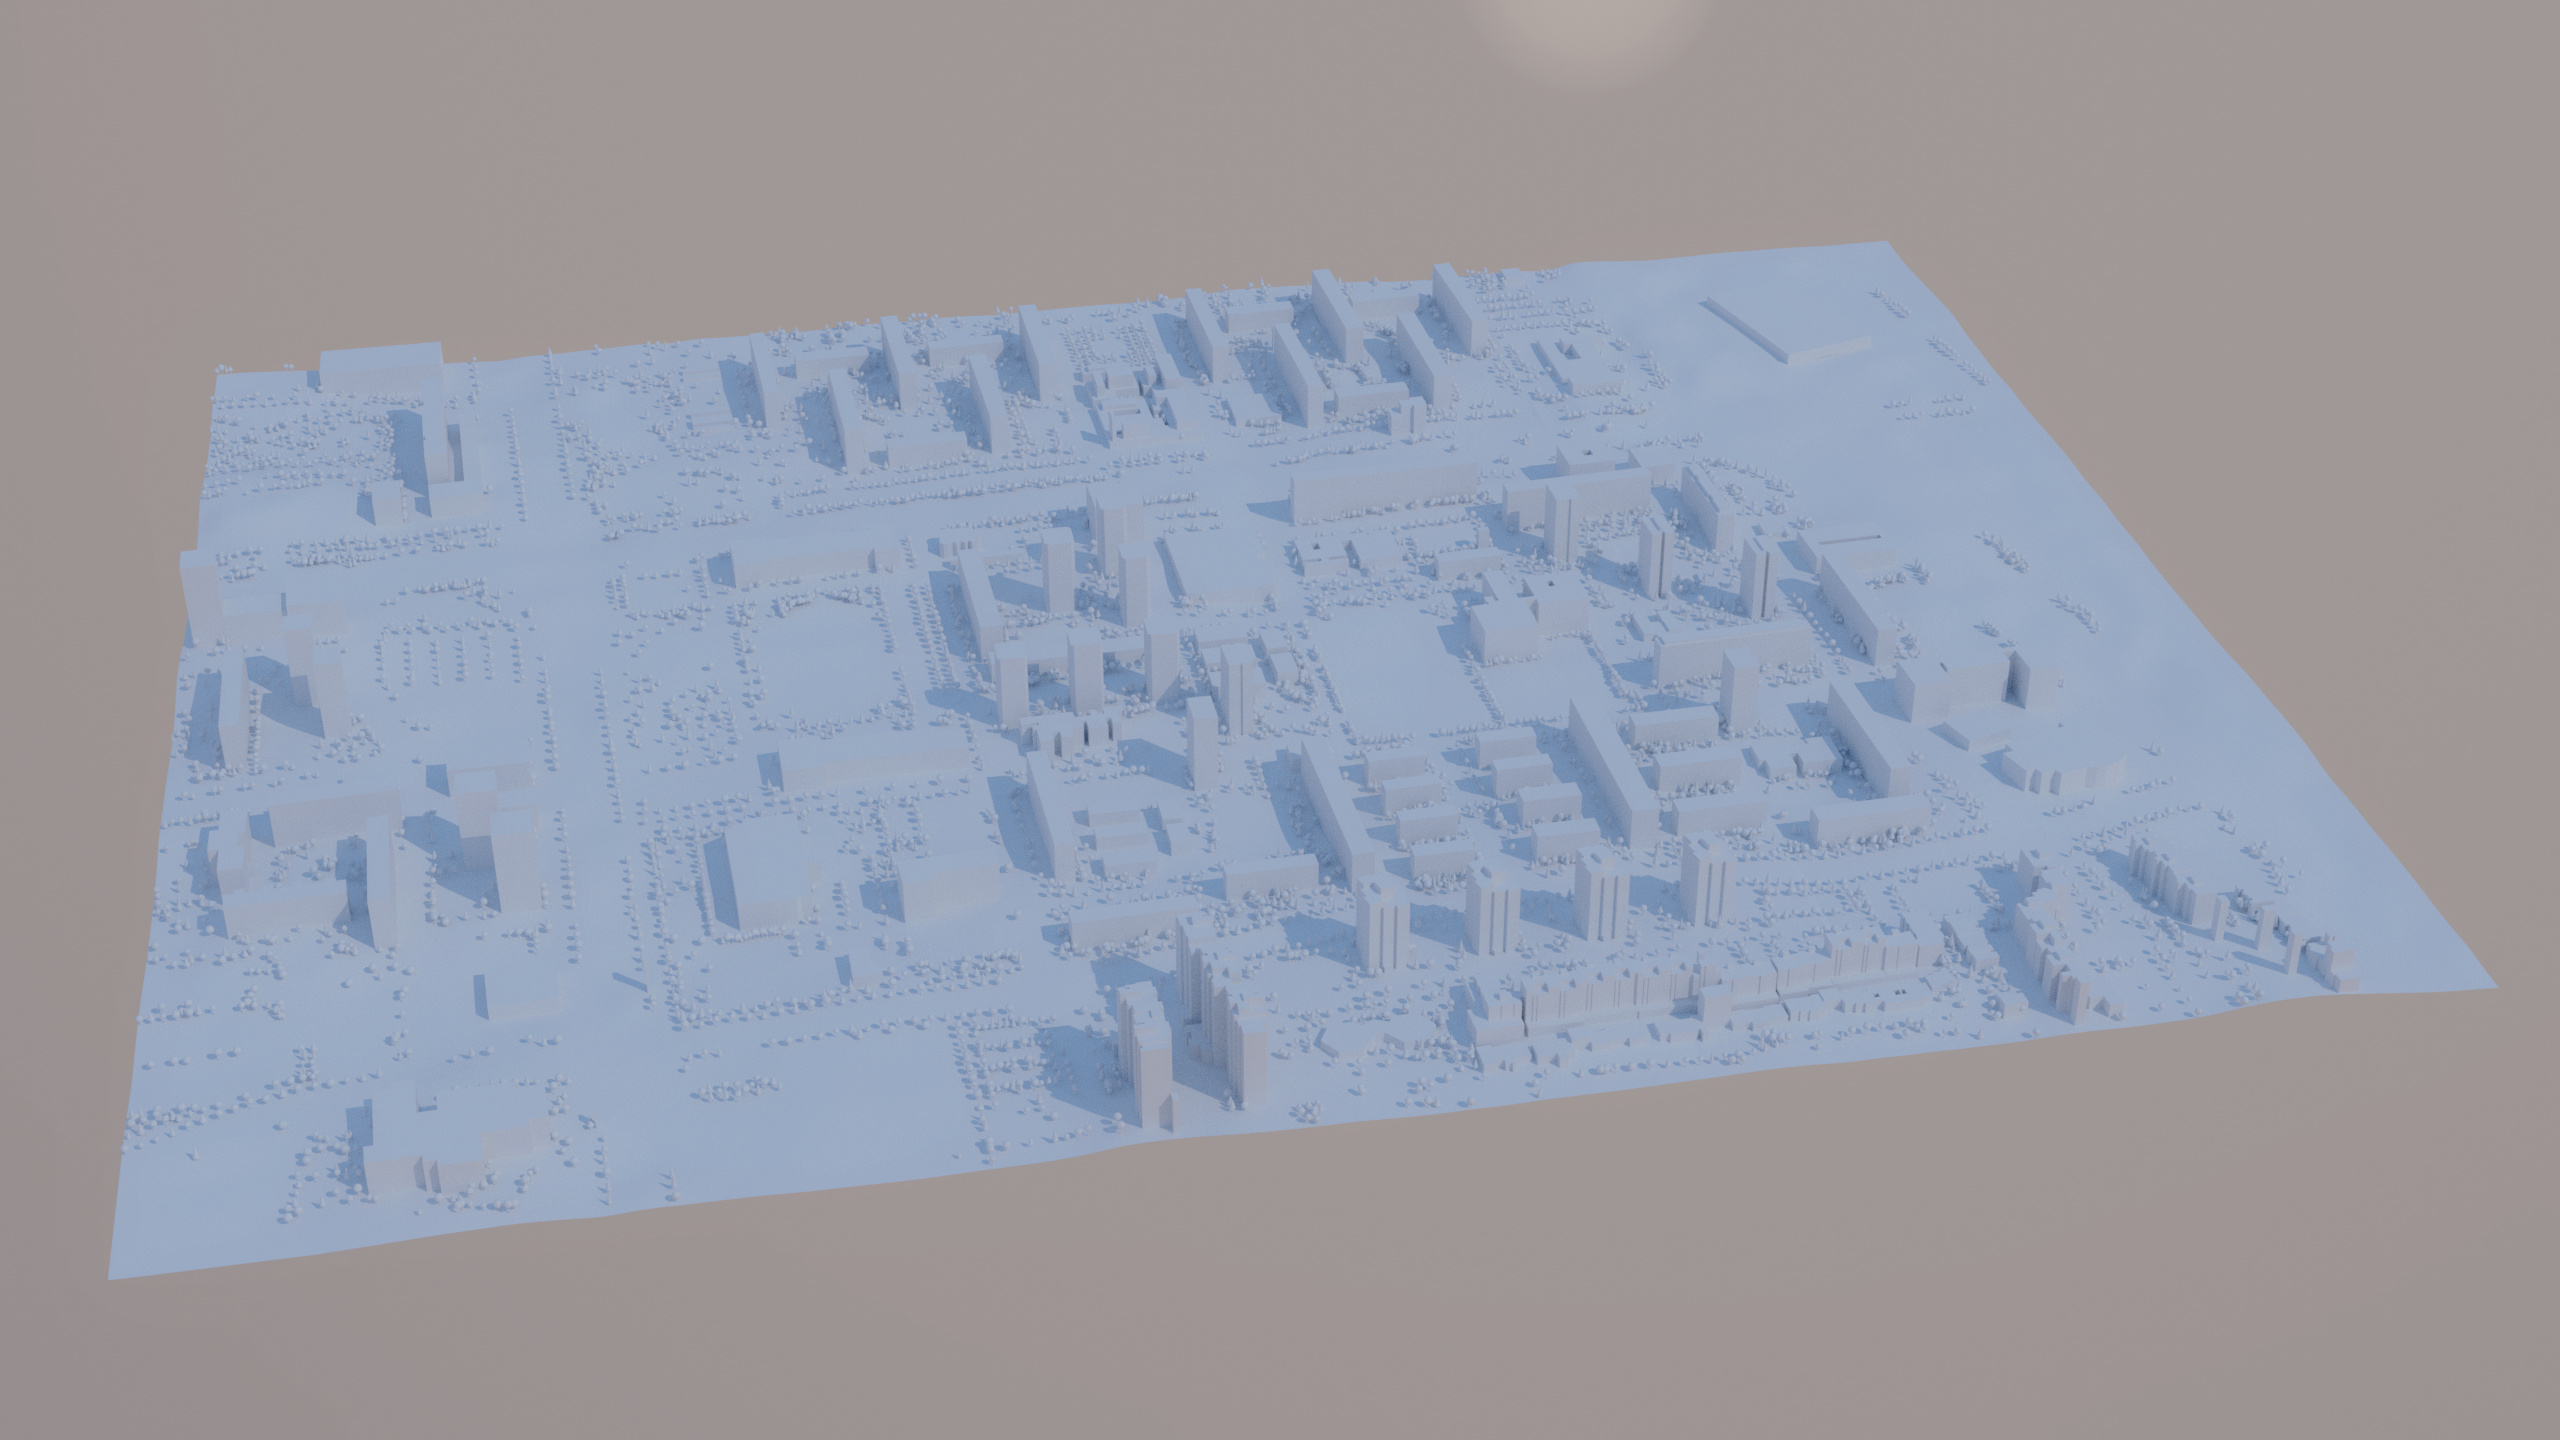
\includegraphics[width=\linewidth]{figures/utrine_entire_render.jpg}
			\caption{Cijela četvrt Utrina i dio okolice}
			\label{fig:utrine_entire_render}
		\end{subfigure}
		\par\bigskip
		\begin{subfigure}{\linewidth}
			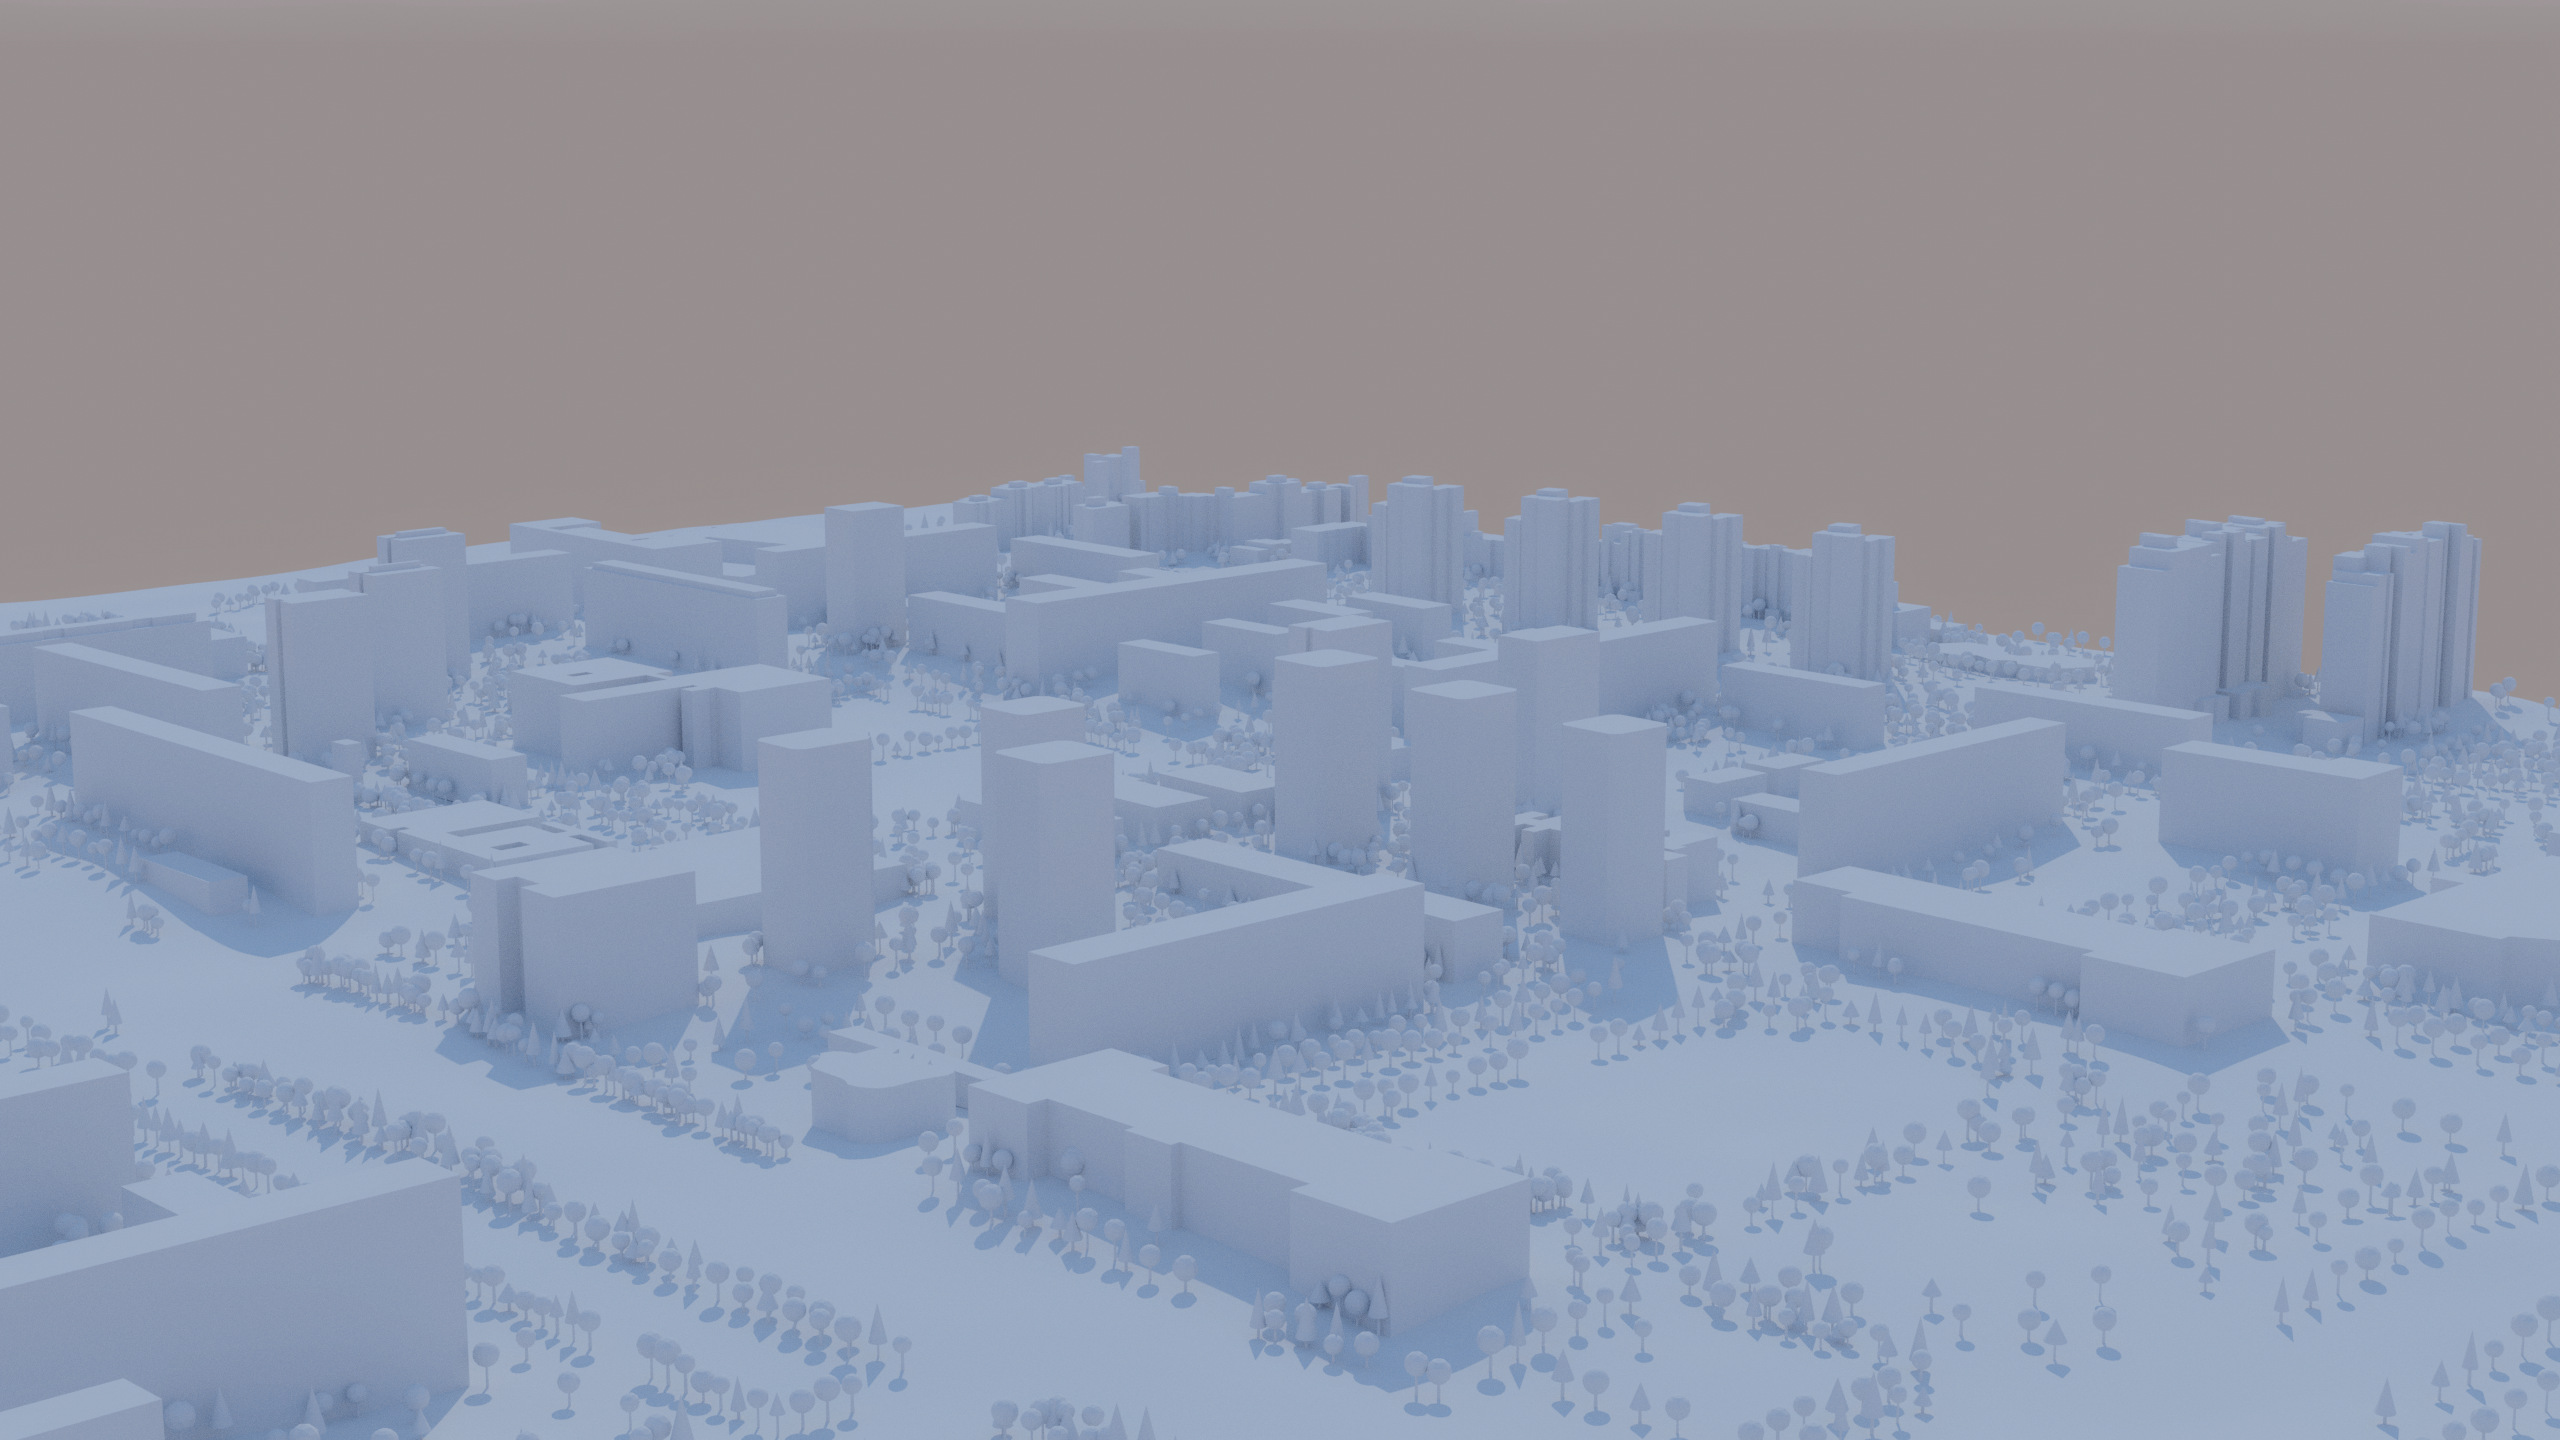
\includegraphics[width=\linewidth]{figures/utrine_detail_render.jpg}
			\caption{Detalj četvrti Utrina}
			\label{fig:utrine_detail_render}
		\end{subfigure}
		\caption{Izrađen prikaz generiranog modela gradske četvrti Utrina}
		\label{fig:utrine_renders}
	\end{figure}
	
	Model gradske četvrti Utrina prikazan na slici \ref{fig:utrine_renders} pokriva površinu od \SI{1.42}{\kilo\meter\squared}.
	Generiranje je trajalo približno \SI{20}{} minuta, od čega je \SI{90}{\percent} vremena utrošeno na stvaranje stabala.
	Ukupno je stvoreno približno \SI{320}{} zgrada i \SI{7 100}{} stabala.
	Cijeli model ima približno \SI{1 455 000}{} trokuta i \SI{757 000}{} vrhova.
	Na slici \ref{fig:utrine_detail_render} uočljivo je da su gotovo sve zgrade i neboderi ispravne visine.
	Takav ishod mogao se i predvidjeti s obzirom na to da je četvrt odlično pokrivena podatcima o visinama zgrada (slika \ref{fig:overpass_zagreb_all_buildings_with_height}).
	
	Generirani model dijela grada može se izvesti \engl{export} iz \textit{Blendera} te primjerice uvesti \engl{import} u \textit{Unreal Engine}.\footnote{\url{https://docs.unrealengine.com/en-US/Engine/Content/Importing/FBX/FullScene/index.html}}
	Upravo je to učinjeno i prikazano na slici \ref{fig:ue4_game_jumping}.
	S lijeve strane može se iz trećeg lica vidjeti model igrača u skoku, dok je s desne strane u pozadini vidljiva Zagrebačka katedrala.
	
	\begin{figure}[H]
		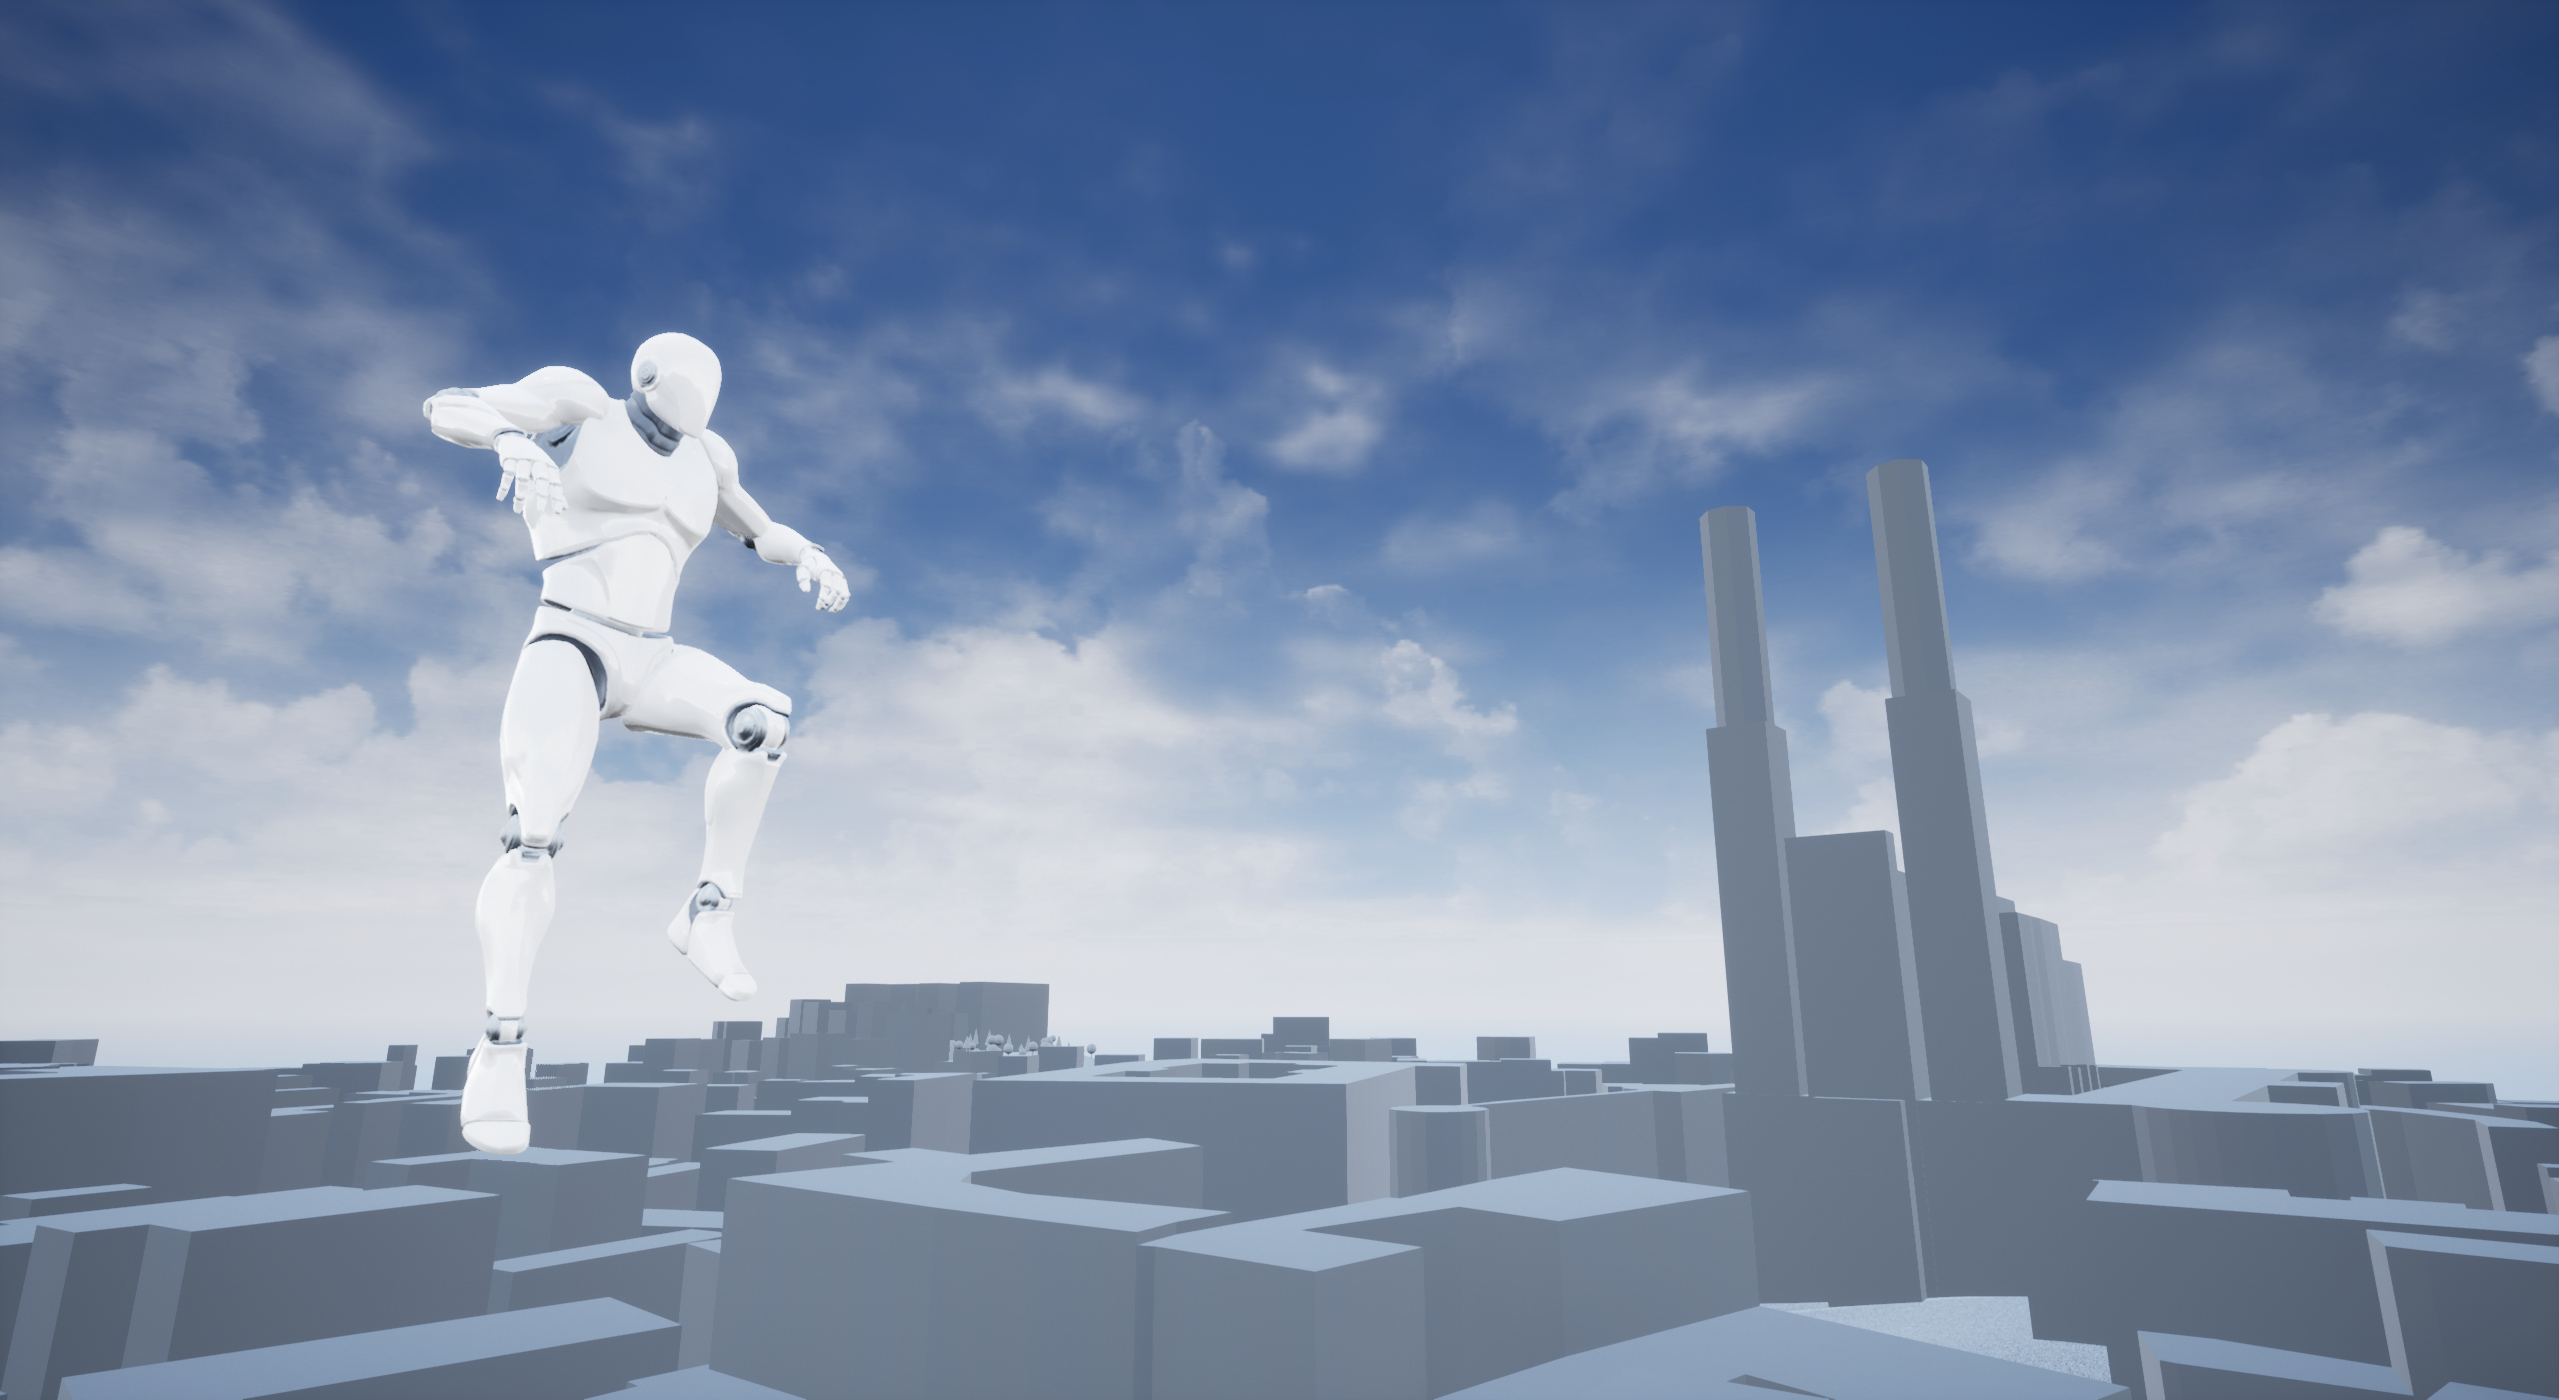
\includegraphics[width=\linewidth]{figures/ue4_game_jumping.jpg}
		\centering
		\caption{Scena iz grafičkog pogona \textit{Unreal Engine}}
		\label{fig:ue4_game_jumping}
	\end{figure}



\chapter{Zaključak}
	
	Rezultat rada jest programsko rješenje koje omogućuje automatiziranu izradu osnovnog modela proizvoljnog dijela grada Zagreba.
	Model u omjeru $1:1$ vjerno prikazuje odabrani dio grada.
	
	Očekivano, ostaje mnogo prostora za poboljšanje.
	Osim stabala, Zrinjevac u svojem Katastru zelenila nudi podatke o grmlju koje održava, kao i urbanoj opremi poput klupa, sprava na dječjim igralištima te koševa za smeće.
	OSM ima podatke o travnjacima, livadama i šumama koji se mogu iskoristiti za točniju reprezentaciju zelenih površina.
	Također, kvaliteta generiranog modela grada značajno bi se poboljšala dodavanjem tekstura, primjerice projiciranjem satelitske snimke na model terena ili teksturiranjem pročelja zgrada.
	Bilo bi poželjno i da krovovi svih zgrada nisu potpuno ravni.
	
	Navedena poboljšanja doprinijela bi boljoj predočivosti i vizualnoj atraktivnosti stvorenog modela.
	Time bi bilo omogućeno učinkovitije urbanističko planiranje pojedinih gradskih četvrti.\\
		
	Programski kôd u cijelosti je javno dostupan na \textit{GitHub} repozitoriju:\\
	\url{https://github.com/LMesaric/BSc-Thesis-FER-2020}



\bibliography{literatura}
\bibliographystyle{fer}



\begin{sazetak}
	
	U ovom radu razmatra se postupak automatskog programskog generiranja trodimenzionalnog modela proizvoljnog dijela grada Zagreba.
	Diskusija je popraćena konkretnom programskom implementacijom rješenja u programskom jeziku \textit{Python} u obliku dodatka za alat \textit{Blender}.
	Model se temelji na realnim i javno dostupnim podatcima o terenu, zgradama i stablima te se izrađuje u omjeru $1:1$.
	Kao izvori podataka opisuju se i koriste NASA-ine satelitske snimke senzorom ASTER, baza prostornih kartografskih informacija \textit{OpenStreetMap} i Katastar zelenila Zagreba.
	Generirani \mbox{model} sastoji se od mreže vrhova i poligona bez teksture kojom su predstavljeni teren, zgrade s ravnim krovovima te stabla.
	
	\kljucnerijeci{3D model grada, 3D geoinformacije, interaktivna vizualizacija, \mbox{Zagreb}, \mbox{OpenStreetMap}, Blender, Python, Unreal Engine}
\end{sazetak}


\engtitle{Zagreb District Model Based on Real Data}
\begin{abstract}
	
	This thesis examines the procedure of automatic computer generation of a three-dimensional model of an arbitrary Zagreb district.
	The discussion is accompanied by the implementation of the solution in software using the \textit{Python} programming language in the form of an add-on for \textit{Blender} toolset.
	The model is based on accurate and publicly available data on terrain, buildings and trees, and is made in $1:1$ ratio.
	NASA's satellite images created using the ASTER sensor, spatial \mbox{geoinformation} \mbox{database} \mbox{\textit{OpenStreetMap}} and the Zagreb Green cadastre are described and used as data sources.
	The generated city model consists of meshes without textures representing the terrain, buildings with flat roofs and trees.
	
	\keywords{3D city model, 3D geoinformation, interactive visualization, \mbox{Zagreb},\\ \mbox{OpenStreetMap}, Blender, Python, Unreal Engine}
\end{abstract}

\end{document}
